% !TEX program = xelatex
\documentclass[UTF8,10pt,a4paper]{ctexart}

% ---------- 页面与宏包 ----------
\usepackage[margin=2.0cm,top=2.0cm,bottom=2.0cm]{geometry}
\usepackage{booktabs}
\usepackage{multirow}
\usepackage{graphicx}
\usepackage{amsmath,amssymb}
\usepackage{caption}
\usepackage{subcaption}
\usepackage{xcolor}
\usepackage{hyperref}
\usepackage{enumitem}
\usepackage{array}
\usepackage{float}
\usepackage{tikz}
\usepackage[ruled,vlined,linesnumbered]{algorithm2e}
\SetAlgorithmName{算法}{算法}{算法列表}
\usetikzlibrary{positioning,arrows.meta,calc}

\setCJKmainfont{SimSun}
\setCJKsansfont{WenQuanYi Micro Hei}
\setCJKmonofont{WenQuanYi Micro Hei Mono}
\captionsetup{font=small,labelfont=bf}
\setlist{nosep,leftmargin=1.4em}
\hypersetup{colorlinks=true,linkcolor=blue!50!black,citecolor=blue!50!black,urlcolor=blue!50!black}
\graphicspath{{../../results/gtzan/figures/}{../../results/fma/figures/}{../../results/token_prediction/figures/}{../../results/generation/figures/}{figures/}}
\newcommand{\MvpCnnF}{0.753}
\newcommand{\MvpAstF}{0.814}
\newcommand{\FmaBestModel}{AST（预训练）}
\newcommand{\FmaBestF}{0.590}
\newcommand{\FmaBestAcc}{0.596}
\newcommand{\FmaTestN}{1199}
\newcommand{\FmaCnnF}{0.470}
\newcommand{\LeakCnnF}{0.568}
\newcommand{\LeakCnnAcc}{0.566}
\newcommand{\LeakDelta}{+9.9}
\newcommand{\AblationSentence}{验证集上最佳配置为 CNN + SpecAug + LS（Macro-F1 0.529），但相对 CNN 基线仅提升 +0.7 个百分点，处于单次运行的波动范围内；因此主实验保留基线配置，不引入额外复杂度。}
\newcommand{\FmaTrackLeak}{971}
\newcommand{\FmaTrackLeakN}{1199}
\newcommand{\FmaTrackLeakPct}{81.0}
\newcommand{\FmaArtistLeak}{0}
\newcommand{\FinetuneSentence}{LoRA（rank 8，alpha 16）在 11192 个训练窗口上以 batch 16 训练 1200 步、约 44.1 分钟，峰值显存 1782\,MB，仅更新 144 个投影层，测试集未参与。目标值从训练初期的 7.60 降到 5.98（均匀分布基准 $\ln 2048=7.62$），即模型确实学到了 Token 层面的结构。}
\newcommand{\TokPersistenceFree}{0.016}
\newcommand{\TokFrequencyFree}{0.012}
\newcommand{\TokBigramFree}{0.017}
\newcommand{\TokLstmFree}{0.021}
\newcommand{\TokLstmNll}{6.559}
\newcommand{\TokLstmTrainS}{992}
\newcommand{\TokTransformerFree}{0.022}
\newcommand{\TokTransformerNll}{6.522}
\newcommand{\TokTfFreeStd}{0.000}
\newcommand{\TokTfTeacher}{0.034}
\newcommand{\TokTfTrainS}{2513}
\newcommand{\TokTfParams}{5.0M}
\newcommand{\TokNTest}{2,398}
\newcommand{\TokNTrain}{11,192}
\newcommand{\TokNTracks}{1,199}
\newcommand{\GenBaseLat}{3.7}
\newcommand{\GenBaseMem}{1393}
\newcommand{\GenBaseRmse}{19.23}
\newcommand{\GenFtVOneNegLat}{4.9}
\newcommand{\GenFtVOneNegMem}{1393}
\newcommand{\GenFtVOneNegRmse}{18.43}
\newcommand{\GenFtLat}{4.4}
\newcommand{\GenFtMem}{1396}
\newcommand{\GenFtRmse}{17.91}
\newcommand{\GenFullLat}{3.1}
\newcommand{\GenFullMem}{1396}
\newcommand{\GenFullRmse}{17.64}
\newcommand{\GenRSixteenLat}{3.1}
\newcommand{\GenRSixteenMem}{1396}
\newcommand{\GenRSixteenRmse}{18.59}
\newcommand{\FtSteps}{1200}
\newcommand{\FtRank}{8}
\newcommand{\FtMinutes}{44}
\newcommand{\FtMem}{1782}
\newcommand{\BudgetSentence}{在 GTZAN 上加长训练的最好增益为 $+0.0136$，而在 FMA-small 上为 $+0.0024$（均值为 $-0.0046$）——这说明主实验的原训练预算已经够用，早停并没有系统性地截断仍在改善的模型；GTZAN 上的小幅提升主要来自小数据集上方差更大的训练过程，不宜据此宣称模型被欠训练。}


\title{\vspace{-1.2cm}\textbf{从传统机器学习到预训练 Transformer：\\音乐流派分类的系统性基准与优化}}
\author{《走进音乐人工智能》课程项目组\\
\small 代码与结果：\url{https://github.com/weiza0v0/music-ai-lab}}
\date{2026 年 10 月}


% ---- 分部标题：article 类的 \part 不换页且编号会串，这里自定义 ----
\newcommand{\projectpart}[1]{%
  \clearpage
  \phantomsection
  \addcontentsline{toc}{part}{#1}%
  \thispagestyle{plain}%
  \vspace*{6em}%
  \begin{center}
    {\Huge\bfseries #1}\par
    \vspace{1.4em}
    {\color{gray}\rule{0.4\linewidth}{0.6pt}}
  \end{center}
  \vspace{3em}
  \clearpage}

\begin{document}
\maketitle

% ================= 摘要 =================
\begin{abstract}
\noindent
音乐流派分类是音乐信息检索的经典任务，也是检验不同建模范式的天然试验台。本文在\emph{同一套数据划分、同一批音频片段与同一套评估协议}下，系统比较了六类模型：基于人工特征的 SVM 与 MLP、端到端 CNN、CNN+BiGRU（CRNN）、轻量 Transformer，以及冻结 AudioSet 预训练主干的 Audio Spectrogram Transformer（AST）。实验覆盖两个数据集：清洗后的 GTZAN（985 首、10 流派，作为最小可行 MVP）与 FMA-small 主实验（8\,000 首、8 流派）。所有深度模型使用 3 个随机种子重复训练，测试集只在模型冻结后评估一次，并启用了 cuDNN 确定性以保证可复现。在 GTZAN 上，从头训练的 CNN 的 Macro-F1 为 0.753；冻结预训练主干的 AST 达到 0.814；在 FMA-small 上最佳模型 AST（预训练） 的 Macro-F1 为 0.590。
本文进一步给出错误分析、七种扰动下的鲁棒性实验、片段级时间轴分析，以及面向 CNN/CRNN/Transformer 的 SpecAugment 与标签平滑优化消融。结果显示：预训练表示带来最大的单点收益，但在噪声与短片段下所有模型的可靠性都显著下降；深度模型赢在干净输入，传统模型在输入变脏时反而更稳。
本文因此分为\textbf{判别式与生成式两个任务}：前者即上述流派分类，后者把预测目标从流派标签换成\textbf{离散 Token 序列}——用 EnCodec 把音频量化成 50\,Hz、4 码本的 Token，比较 LSTM 与小 Transformer 对下 1 秒 Token 的预测能力，并评估 MusicGen-small 的前缀续写与 LoRA 适配。该部分记录了一次\textbf{被修正的负结果}：初版 LoRA 适配因标签维度错误而完全无效（目标值停在均匀分布之上），修正后音频距离从 19.23 降到 17.91，且 8 首中 7 首改善——说明"训不动"未必是容量或数据不足，也可能只是目标对齐写错了。
代码、权重生成脚本与全部结果文件均已开源。
\vspace{0.3em}\\
\textbf{关键词：}音乐流派分类；GTZAN；FMA-small；卷积神经网络；CRNN；Transformer；迁移学习；可复现实验
\end{abstract}

\newpage
\tableofcontents
\newpage

% ================= 1 引言 =================
\section{引言}

\subsection{研究背景}

音乐流派（genre）是人类对音乐风格的一种高层概括，广泛用于推荐、检索、曲库管理与版权结算。自动流派分类要求模型从波形中提取音色、节奏、和声与配器等线索，是连接信号处理与音乐理解的典型任务\cite{tzanetakis2002gtzan,casey2008content}。在流媒体平台上，每天有大量新曲目缺少人工标注，自动流派标签能显著降低冷启动成本；在音乐教育中，流派分类也可以作为理解音色与节奏的入口。

过去十余年，该任务的建模路线经历了三次明显的迁移：从人工特征加浅层分类器，到端到端卷积网络\cite{choi2017crnn,dieleman2014endtoend}，再到自注意力\cite{vaswani2017attention}与大规模预训练模型\cite{gong2021ast,kong2020panns}。每一次迁移都伴随新的问题：深度模型是否真的优于精心设计的人工特征？预训练带来的收益有多少来自数据、多少来自架构？在资源受限的课堂上，我们能否得到可信、可复现的结论？

与分类这条线并行的，是近三年兴起的\textbf{生成式}路线。其关键一步是把连续波形离散化：
神经音频编解码器（SoundStream、EnCodec\cite{defossez2023encodec}）用残差向量量化把音频压成
每秒几十帧、每帧若干个码本的离散 Token。一旦音频变成 Token 序列，"下一个 Token 是什么"
就成为一个可以用交叉熵直接度量的语言建模问题——AudioLM\cite{borsos2023audiolm} 据此做音频续写，
MusicGen\cite{copet2023musicgen} 进一步把文本条件接进来，成为可控的音乐生成模型。
这条路线带来一个诱人的猜想：如果同一个系统既能把音频压成 Token，又能预测 Token，
那么"理解音乐"与"生成音乐"或许是同一件事的两面。

本文因此在流派分类之外，用\textbf{同一批数据与同样严格的划分纪律}再做一个生成式任务：
在离散 Token 层面预测真实未来、把预测解码回音频、并评估预训练生成模型的前缀续写。
两个任务并列，而不是把生成当作分类的附属演示。

\subsection{问题与挑战}

文献中的准确率数字往往不可直接比较，原因至少包括：
\begin{enumerate}
  \item \textbf{数据划分不一致}：同一数据集的不同版本、不同随机划分，甚至测试集被反复用于调参；
  \item \textbf{片段与预处理不一致}：3 秒 / 5 秒 / 10 秒片段、采样率、归一化方式都会改变输入分布；
  \item \textbf{标签本身模糊}：「Rock」与「Metal」、「Pop」与「Dance」的边界在人类标注者之间也不一致；
  \item \textbf{数据泄漏隐蔽}：同一曲目的不同片段、同一艺术家的不同作品跨集合，都会让模型「记住来源」而不是学习风格；
  \item \textbf{计算预算差异}：预训练模型的权重体积与推理延迟比自建模型高两到三个数量级。
  \item \textbf{生成任务没有唯一的正确答案}：分类有明确标签可以对齐，而"这段前缀之后应当
        是什么"本身是开放集合。用与真实后续的距离（如 Log-Mel RMSE 或 FAD\cite{kilgour2019fad}）
        度量，只能说明"接近真实"而非"好听"；主观评分又难以规模化。因此生成实验必须
        明确区分\textbf{可度量的部分}（Token 级 NLL、Top-1）与\textbf{只能定性判断的部分}（音乐性）。
\end{enumerate}
因此，一个负责任的基准必须同时报告\emph{协议、成本与失败模式}，而不只是一个准确率。

\subsection{研究问题}

本文围绕三个问题展开：
\begin{enumerate}
  \item 在完全相同的协议下，不同代际的模型（传统 ML、CNN、CRNN、Transformer、预训练 AST）差距究竟有多大？
  \item 数据规模从千首级（GTZAN）扩大到万首级（FMA-small）时，结论是否稳定？
  \item 常见优化手段（SpecAugment、标签平滑、dropout）能带来多少真实收益，代价是什么？
  \item 把目标从流派标签换成离散 Token 序列后，同一套小容量模型与评估纪律能得到什么？
        8\,GB 显存的课堂上，预训练生成模型的前缀续写与轻量适配各自能做到哪一步，
        失败的边界又在哪里？
\end{enumerate}

\subsection{主要贡献}

本文的主要贡献如下：
\begin{itemize}
  \item \textbf{统一基准}：在同一套按曲目 / 按艺术家划分、同一批 5 秒中心片段、同一套预处理与评估协议下，比较六个代表性模型；
  \item \textbf{泄漏诊断}：量化了 FMA-small 上「按曲目划分」带来的艺术家级泄漏，并用对照实验证明其会把 CNN 的 Macro-F1 虚高约 9.9 个百分点；
  \item \textbf{优化消融}：系统尝试 SpecAugment、标签平滑与 dropout，报告了一个诚实的负结果——在 FMA 上最大提升仅 0.7 个百分点；
  \item \textbf{行为分析}：给出错误分析、七种扰动的鲁棒性、片段级时间轴与置信度校准，说明准确率之外的模型差异；
  \item \textbf{可复现交付}：公开代码、配置、结果文件与 LaTeX 报告，所有数字可由脚本重新生成，且经过独立只读审计。
  \item \textbf{生成式任务基准}：用 EnCodec 把音频量化为 $4\times300$ Token，在同一份
        按艺术家分离的划分上比较 Persistence、频率先验、Bigram 与两种神经模型（LSTM、
        小 Transformer），并\textbf{分别}报告 teacher-forced 与 free-running 两种口径，
        避免用前者冒充后者。
  \item \textbf{一次被修正的负结果}：预训练生成模型的 LoRA 适配初版完全无效。我们用
        未训练模型的目标值对照（错误布局 11.08 / 正确布局 5.46 / 均匀分布 7.62）定位到
        标签维度错误，修正后音频距离由 19.23 降到 17.91 且 8 首中 7 首改善；而随后
        对训练步数、目标窗口、适配秩三个旋钮的配对检验\textbf{均不显著}。
  \item \textbf{负结果的辨别方法}：本文给出三件在报告中容易被忽略的检验——逐曲配对检验
        （排除"单首拉低均值"）、去掉最优样本后的复核、以及按几何衰减外推判断"最优轮次
        撞上限"是否真的意味着欠训练。三者都曾改变本文的结论。
\end{itemize}

\subsection{报告组织}

第~\ref{sec:related} 节回顾相关工作；第~\ref{sec:data} 节介绍数据与预处理协议。此后正文分为\textbf{三个部分}。\textbf{第一部分}处理判别式任务：第~\ref{sec:method} 节给出模型、训练方法与实验设置，第~\ref{sec:results} 节报告 GTZAN 与 FMA-small 的结果、消融，以及错误、鲁棒性与片段级分析。\textbf{第二部分}处理生成式任务：第~\ref{sec:phase2} 节把目标从流派标签换成离散 Token 序列，依次给出 Token 化协议、预测模型、预测结果、解码验证，以及预训练生成模型的前缀续写与轻量适配。\textbf{第三部分}是综合讨论：第~\ref{sec:discussion} 节汇总主要发现、解释性分析与局限，第~\ref{sec:conclusion} 节总结。附录给出逐 seed 结果、完整超参与复现命令。

% ================= 2 相关工作 =================
\section{相关工作}\label{sec:related}

\subsection{音乐信息检索与流派分类}

音乐信息检索（Music Information Retrieval, MIR）关注从音频、乐谱、歌词或元数据中提取结构化信息\cite{downie2003mir,casey2008content}。流派分类是其中最早被系统研究的任务之一：Tzanetakis 与 Cook 在 2002 年提出用谱特征、节奏特征与梅尔倒谱系数训练分类器，并发布了 GTZAN 数据集\cite{tzanetakis2002gtzan}。此后二十年，该任务逐渐成为检验新表示与新架构的标准试验台。

\subsection{人工特征与浅层模型}

传统方法通常把音频切帧，逐帧计算 MFCC、谱质心、谱带宽、rolloff、过零率、chroma 与节奏直方图，再在时间维做统计池化，最后送入 SVM、随机森林或 k 近邻\cite{tzanetakis2002gtzan,bogdanov2013essentia}。这类方法有两个优点：一是计算便宜，二是特征具有明确的声学含义。其局限在于统计池化会丢失时间结构，且特征设计依赖领域知识。

\subsection{端到端深度模型}

随着数据规模与算力增长，端到端学习逐渐取代人工特征。Dieleman 与 Schrauwen 直接把波形送入 CNN\cite{dieleman2014endtoend}；Choi 等提出 CRNN，用卷积层提取局部时频模式、用循环层建模时间演化\cite{choi2017crnn}；Humphrey 等系统比较了特征学习与手工特征\cite{humphrey2013feature}。在音频事件识别领域，Hershey 等比较了多种 CNN 架构\cite{hershey2017cnn}，PANNs 则用大规模预训练提升通用性\cite{kong2020panns}。

\subsection{Transformer 与预训练}

Transformer 的自注意力机制\cite{vaswani2017attention}能建模长程依赖，Vision Transformer 把图像切 patch 后直接用 Transformer 编码。AST 把这一思路迁移到音频：将 Log-Mel 频谱切成 $16\times16$ 的 patch，在 AudioSet\cite{gemmeke2017audioset}上预训练，再迁移到下游分类任务\cite{gong2021ast}。在小数据场景，冻结主干、只训练线性分类头是常见策略，但其收益同时来自预训练数据与架构，两者需要分开讨论。

\subsection{数据集与评测偏差}

GTZAN\cite{tzanetakis2002gtzan} 是最常用的基准，但 Sturm 指出其存在重复音频、标签错误、失真与艺术家泄漏等问题，容易高估模型能力\cite{sturm2013gtzan}。FMA\cite{defferrard2017fma} 提供了规模更大、授权更清晰的替代数据；MSD\cite{bertin2011msd} 则侧重百万级曲目与元数据。本文选择 GTZAN 作为快速验证集、FMA-small 作为主实验集，并对两者都做泄漏检查。

\subsection{鲁棒性与可复现性}

真实部署中的音频会经历音量变化、噪声、压缩与片段截断。已有工作表明，音频分类模型对这些扰动并不稳健，且不同特征表示（绝对 dB 与归一化 dB）的敏感性差异很大。本文用七种扰动系统评测五个模型，并把可复现性作为一等公民：固定种子、确定性 kernel、自动化协议测试与独立审计。

\subsection{离散音频 Token 与音乐生成}

要把音乐生成交给语言模型，第一步是把连续波形变成离散序列。SoundStream 与
EnCodec\cite{defossez2023encodec} 用残差向量量化（RVQ）把音频压成低帧率的码本序列：
EnCodec 在 32\,kHz 上以 50\,Hz 输出 4 个码本、每个码本 2048 个词表项，码率约 2.2\,kbps，
解码后的听感仍接近原始音频。这一步的意义不只是压缩——它让音频与文本一样，成为
"可以用交叉熵预测的离散序列"。

AudioLM\cite{borsos2023audiolm} 直接利用这一点：把音频分成语义 Token 与声学 Token 两级，
用 Transformer 做自回归续写，得到长时间尺度的连贯音频。MusicLM 把文本条件加入同一框架。
MusicGen\cite{copet2023musicgen} 做了简化：单阶段 Transformer 直接建模 EnCodec 的多个码本，
用\textbf{delay pattern} 把并行的码本流错开一帧、拼成一条序列，从而用一个因果语言模型
同时处理多个码本；其 small 版本约 300\,M 参数，是本项目在 8\,GB 显存上唯一可行的选择。
本项目的生成式任务沿用这套 Token 格式，因此需要先实测本环境的 EnCodec 与
MusicGen 权重是否真的互操作（能解码回放才算兼容），而不是假设"同系列即可互换"。

在适配层面，全量微调一个 300\,M 的生成模型对 8\,GB 显存并不划算。LoRA\cite{hu2021lora}
冻结原始权重、只训练低秩旁路（$W+\frac{\alpha}{r}BA$），把可训练参数压到原来的千分之一量级，
是资源受限场景的常见选择。需要注意的是，LoRA 只降低\textbf{优化成本}，并不保证目标对齐正确——
本文的生成式任务正是在这一点上踩过一个不报错的坑。

生成任务的评价本身仍有争议。Fréchet Audio Distance\cite{kilgour2019fad} 等参考无关指标
用预训练嵌入的分布距离度量"像不像真实音乐"，但它与人类主观判断的相关性并不稳定；
与真实后续的频谱距离（本文采用的 Log-Mel RMSE）则只衡量"接近这段真实音频"，
不衡量音乐性。因此本文把 Token 级指标、音频级距离与定性试听分开报告，不把任何一个
单独当成"生成质量"。

% ================= 3 数据与协议 =================
% ================= 3 数据与协议 =================
\section{数据与实验协议}\label{sec:data}

\subsection{GTZAN（MVP 数据集）}
GTZAN 包含 10 个流派各 100 首、每首约 30 秒、22\,050\,Hz 单声道音频。审计发现 1 首无法解码（\texttt{jazz.00054}），28 首与其他曲目 MD5 完全相同。我们剔除损坏文件，并对重复组只保留第一首，最终得到 \textbf{985 首}。按曲目分层划分 70/15/15（689/149/147），随机种子 42。逐流派统计见表~\ref{tab:gtzan-data}。

\begin{table}[H]
\centering\small
\caption{GTZAN 清洗后的逐流派统计。}
\label{tab:gtzan-data}
\begin{tabular}{lccc}
\toprule
流派 & 曲目数 & 平均时长 (s) & 采样率\\
\midrule
blues & 100 & 30.01 & 22,050\\
classical & 100 & 30.03 & 22,050\\
country & 100 & 30.02 & 22,050\\
disco & 99 & 30.02 & 22,050\\
hiphop & 98 & 30.08 & 22,050\\
jazz & 99 & 30.03 & 22,050\\
metal & 93 & 30.00 & 22,050\\
pop & 98 & 30.00 & 22,050\\
reggae & 99 & 30.01 & 22,050\\
rock & 99 & 30.02 & 22,050\\
合计 & 985 & 30.02 & --\\
\bottomrule
\end{tabular}
\end{table}


GTZAN 的优点是规模小、类别均衡、加载快；缺点是标签噪声与重复音频，且缺少可靠的艺术家元数据（原始文件仅以文件名区分曲目）。因此它适合做快速迭代与教学演示，不适合作为唯一证据。

\subsection{FMA-small（主实验数据集）}
FMA-small 包含 8\,000 首、8 个均衡流派的 30 秒片段，原始采样率 44.1\,kHz。初步按曲目分层 70/15/15 划分后，我们做了艺术家级泄漏检查，发现测试集中 \FmaTrackLeak{} / \FmaTrackLeakN{} 首（\FmaTrackLeakPct\%）与训练集共享艺术家——同一乐队的作品在音色、录音与编曲上高度相似，这会让模型「认出乐队」而不是「听懂流派」。因此主实验改用\textbf{按艺术家分离}的划分（每位艺术家整体进入且仅进入一个集合，测试集与训练集的艺术家重叠为 0），并按流派保持大致比例（由于艺术家作品数不均，逐类比例并不完全相等，见附录表~\ref{tab:data}）。曲目级划分保留为泄漏对照实验。数据审计还发现 6 首损坏音频（与官方 SHA1 清单一致，属上游数据问题）与 4 首中心 5 秒数字静音的曲目；前者剔除，后者保留并在附录中说明。艺术家分离划分的逐流派数量见表~\ref{tab:fmasplit}。

\begin{table}[H]
\centering\small
\caption{FMA-small 艺术家分离划分的逐流派数量。}
\label{tab:fmasplit}
\begin{tabular}{lccc}
\toprule
流派 & 训练 & 验证 & 测试\\
\midrule
Electronic & 726 & 134 & 139\\
Experimental & 733 & 119 & 147\\
Folk & 614 & 249 & 137\\
Hip-Hop & 694 & 168 & 135\\
Instrumental & 792 & 82 & 126\\
International & 650 & 194 & 156\\
Pop & 689 & 120 & 191\\
Rock & 698 & 133 & 168\\
合计 & 5596 & 1199 & 1199\\
\bottomrule
\end{tabular}
\end{table}


需要强调，艺术家分离划分不是「免费」的：由于部分艺术家拥有大量作品（最多的一个艺术家有 208 首），划分后逐流派的验证/测试比例并不完全相等（例如 Folk 的验证集 249 首、Instrumental 的验证集 82 首）。这会轻微影响早停与阈值选择，但测试集仍有 126--191 首/类，宏平均指标对类别比例不敏感。

\subsection{统一预处理}
所有模型使用\textbf{每首曲目中心 5 秒}片段，重采样到 22\,050\,Hz 单声道。传统模型输入 209 维人工特征，深度模型输入 $64\times216$ 的 Log-Mel 频谱：
\begin{equation}
  S_{\mathrm{dB}}(m,t)=10\log_{10}\!\left(\sum_{f} |X(f,t)|^{2}\,H_{m}(f)\right),\qquad
  \tilde{S}=S_{\mathrm{dB}}-\max_{m,t} S_{\mathrm{dB}},
\end{equation}
其中 $H_m$ 为 64 个 Mel 滤波器，$|X(f,t)|^2$ 为短时傅里叶功率谱（$n_{\text{fft}}=1024$，hop$=512$）。以片段最大值为参考的归一化使表示对整体增益不敏感，这一点在鲁棒性实验中会再次出现。

209 维人工特征的组成见表~\ref{tab:features}。所有统计量在时间维做均值与标准差池化；标准化器只在训练集拟合。

\begin{table}[H]
\centering\small
\caption{209 维人工特征的组成。}
\label{tab:features}
\begin{tabular}{llc}
\toprule
特征组 & 说明 & 维度\\
\midrule
MFCC（40） & 均值 + 标准差 & 80\\
$\Delta$MFCC（40） & 一阶差分的均值 + 标准差 & 80\\
Chroma（12） & 音高类能量均值 + 标准差 & 24\\
谱对比度（7） & 均值 + 标准差 & 14\\
谱形状（3） & 质心、带宽、rolloff 的均值 + 标准差 & 6\\
过零率 & 均值 + 标准差 & 2\\
RMS 能量 & 均值 + 标准差 & 2\\
Tempo & 估计值（归一化） & 1\\
\midrule
合计 & & 209\\
\bottomrule
\end{tabular}
\end{table}

\begin{figure}[H]
  \centering
  \resizebox{\linewidth}{!}{%
  \begin{tikzpicture}[font=\small, >=Stealth, line cap=round, line join=round,
      box/.style={draw=black!55, rounded corners=2pt, align=center,
                  inner sep=4pt, minimum height=12mm},
      feat/.style={box, fill=blue!7, minimum width=3.2cm},
      model/.style={box, fill=orange!9, minimum width=3.0cm},
      data/.style={box, fill=gray!10, minimum width=2.6cm},
      eval/.style={box, fill=green!8, minimum height=36mm, minimum width=3.3cm}]

    % 节点：x 坐标显式排布，保证三条支路等距
    \node[data]  (data) at (0.0,0)    {GTZAN 985 首\\FMA-small 7,994 首};
    \node[box, minimum width=2.9cm] (prep) at (3.4,0)
        {中心 5 秒片段\\22,050 Hz 单声道};

    \node[feat]  (fhand) at (7.4,2.4)  {209 维人工特征\\（MFCC / 谱 / 节奏）};
    \node[feat]  (fmel)  at (7.4,0)    {64\,$\times$\,216 Log-Mel\\（增益归一化）};
    \node[feat]  (fast)  at (7.4,-2.4) {16 kHz 补零 10.24 s\\AST 频谱};

    \node[model] (mhand) at (10.9,2.4)  {SVM / MLP};
    \node[model] (mdeep) at (10.9,0)    {CNN / CRNN /\\轻量 Transformer};
    \node[model] (mast)  at (10.9,-2.4) {冻结 AST\\+ 线性分类头};

    \node[eval]  (eval)  at (15.0,0)   {统一评估协议\\[2pt]
                                       按曲目 / 艺术家划分\\[2pt]
                                       验证集选型\\[2pt]
                                       测试集单次评估\\[2pt]
                                       Acc / Macro-F1 / 成本};

    % 数据 -> 预处理
    \draw[->] (data.east) -- (prep.west);

    % 分发母线：一条水平线 + 一条竖线，再分别进入三条支路
    \coordinate (pbus) at (5.05,0);
    \coordinate (ptop) at (5.05,2.4);
    \coordinate (pbot) at (5.05,-2.4);
    \draw (prep.east) -- (pbus);
    \draw (ptop) -- (pbot);
    \draw[->] (ptop) -- (fhand.west);
    \draw[->] (pbus) -- (fmel.west);
    \draw[->] (pbot) -- (fast.west);

    % 特征 -> 模型
    \draw[->] (fhand.east) -- (mhand.west);
    \draw[->] (fmel.east)  -- (mdeep.west);
    \draw[->] (fast.east)  -- (mast.west);

    % 汇流母线：三个模型先并入竖线，再用单箭头进入评估
    \coordinate (ctop) at (12.75,2.4);
    \coordinate (cmid) at (12.75,0);
    \coordinate (cbot) at (12.75,-2.4);
    \draw (mhand.east) -- (ctop);
    \draw (mdeep.east) -- (cmid);
    \draw (mast.east)  -- (cbot);
    \draw (ctop) -- (cbot);
    \draw[->] (cmid) -- (eval.west);

    % 母线交点：用实心圆点标明「连接」而不是「交叉」
    \fill[black!70] (pbus) circle (0.055);
    \fill[black!70] (cmid) circle (0.055);

  \end{tikzpicture}}
  \caption{统一的实验流程：同一份按曲目（FMA 按艺术家）划分的数据，经分发母线进入人工特征、
  Log-Mel 与 AST 三条支路，再由汇流母线进入统一评估协议；三条支路共享同一批 5 秒中心片段，
  所有预处理只在训练集上拟合。}
  \label{fig:pipeline}
\end{figure}

\subsection{划分协议与泄漏诊断}\label{sec:leakage}

FMA-small 的元数据包含艺术家字段。我们先用常规的按曲目分层划分，然后检查测试集与训练集的艺术家重叠：\FmaTrackLeak{} / \FmaTrackLeakN{} 首（\FmaTrackLeakPct\%）测试曲目与训练集共享至少一位艺术家。同一乐队的作品在音色、录音设备与编曲习惯上高度相似，这会为模型提供一条「认乐队」而非「听懂流派」的捷径。

因此主实验采用按艺术家分离的划分：每位艺术家整体进入且仅进入一个集合。表~\ref{tab:leak} 对比两种划分。可以看到，曲目级划分把 CNN 的 Macro-F1 从 0.470 抬到 0.568（+9.9 个百分点），而输入特征、模型与训练超参完全相同——这正是数据泄漏的典型表现。

\begin{table}[H]
\centering\small
\caption{曲目级划分与艺术家分离划分的对比（FMA-small，CNN seed 42）。}
\label{tab:leak}
\begin{tabular}{lccccc}
\toprule
划分方式 & train / val / test & 测试-训练共享艺术家 & Acc & Macro-F1 & 结论\\
\midrule
按曲目 & 5,595 / 1,200 / 1,199 & 971（81.0\%） & 0.566 & 0.568 & 高估\\
按艺术家 & 5,596 / 1,199 / 1,199 & 0（0.0\%） & 0.480 & 0.470 & 主表采用\\
\bottomrule
\end{tabular}
\end{table}

\subsection{防泄漏与可复现约束}
\begin{itemize}
  \item \textbf{先按曲目划分，再切片}，同一曲目绝不跨集合；
  \item StandardScaler 与 Log-Mel 归一化统计量\textbf{只在训练集上拟合}；
  \item 模型选择只看验证集 Macro-F1，测试集在模型冻结后\textbf{只评估一次}；
  \item FMA 主实验按\emph{艺术家}划分，避免同乐队跨集合；并用曲目级划分做泄漏对照；
  \item 固定种子（42/123/2024），开启 cuDNN 确定性，同种子重跑得到逐字节一致的权重；
  \item 协议由 \texttt{tests/test\_protocol.py} 自动校验，并由独立审计复核。
\end{itemize}

\subsection{两个任务的协议共享与差异}\label{sec:twotask}

判别式与生成式两个任务共用同一份数据与同一条纪律，但在输入格式与评价口径上分道扬镳。
表~\ref{tab:twotask} 汇总了两者的对应关系。

\begin{table}[H]
\centering\small
\caption{两个任务在协议上的共享项与差异项。共享项保证"同一套纪律"，差异项说明为什么
两者的指标不能直接比较。}
\label{tab:twotask}
\begin{tabular}{lll}
\toprule
维度 & 判别式任务 & 生成式任务 \\
\midrule
数据来源 & FMA-small（同 GTZAN 作 MVP） & 同一份 FMA-small \\
划分 & 按艺术家分离，5{,}596/1{,}199/1{,}199 & \textbf{完全复用}同一份划分 \\
测试集使用 & 冻结后评一次 & 冻结后评一次 \\
种子 & 42 / 123 / 2024 & 42 / 123 / 2024 \\
\midrule
输入 & 5\,s 中心片段，22.05/16\,kHz & 6\,s 窗口，32\,kHz 单声道 \\
表示 & 209 维人工特征 + $64\times216$ Log-Mel & $4\times300$ 离散 Token（50\,Hz） \\
输出 & 10 或 8 类标签 & 4 个码本的 Token 序列 \\
指标 & Accuracy、Macro-F1、混淆矩阵 & NLL、Top-1（两种口径）、Log-Mel RMSE \\
\bottomrule
\end{tabular}
\end{table}

需要强调两点。其一，划分严格复用意味着两个任务的测试曲目\textbf{完全相同}——因此
"分类器认对了这首歌"与"模型能续写这首歌"是对同一批曲目的两种提问，结论才有可比性。
其二，两者指标\textbf{不可直接比较}：Macro-F1 是"答对多少"，NLL 是"分布有多接近"，
Log-Mel RMSE 是"生成的频谱与真实未来差多远"。本文在任何地方都不做跨任务的数值比较。

生成式任务的窗口构造有其特殊性：先在曲目/艺术家层面划集合，再在曲目内部切窗，
本次采用每首 2 个 6\,s 窗口（前 5\,s 作前缀、后 1\,s 作预测目标），共 15{,}988 个窗口。
窗口继承曲目所属的集合，因此不存在同一首歌的窗口跨越训练/测试的泄漏。

% ================= 4 方法 =================
\projectpart{I\quad 判别式任务：音乐流派分类}
\section{方法与实验设置}\label{sec:method}\label{sec:setup}

\subsection{传统基线：SVM 与 MLP}
SVM 使用 RBF 核（$C=10$，$\gamma=$scale），MLP 为两层全连接（256-128，ReLU，Adam，early stopping）。二者共享同一份 209 维特征，标准化器仅在训练集拟合。

\subsection{CNN}
输入 $1\times64\times216$ 的 Log-Mel。网络由 4 个卷积块组成，每块含两个 $3\times3$ 卷积、BatchNorm、ReLU 与 $2\times2$ 最大池化，通道数依次为 32/64/128/128；随后自适应平均池化到 $2\times4$，dropout 后接线性分类头，参数量约 59 万。三个自建深度模型的层结构与参数量见表~\ref{tab:arch}。

\begin{table}[H]
\centering\small
\caption{自建模型的层结构与参数量（GTZAN 10 类；括号内为 FMA 8 类的差异）。}
\label{tab:arch}
\begin{tabular}{llc}
\toprule
模型 & 关键层（输入 $\rightarrow$ 输出） & 参数量\\
\midrule
CNN & Conv3$\times$3(32)$\times$2 $\rightarrow$ Pool & \multirow{3}{*}{592,554}\\
    & Conv3$\times$3(64)$\times$2 $\rightarrow$ Pool & \\
    & Conv3$\times$3(128)$\times$2 $\rightarrow$ Pool$\times$2 & \\
    & AdaptiveAvgPool(2,4) $\rightarrow$ FC(1024,10) & \\
\midrule
CRNN & Conv(32/64/128) $\rightarrow$ BiGRU(96) & \multirow{2}{*}{418,986}\\
     & 时间平均 $\rightarrow$ FC(192,10) & \\
\midrule
Transformer & Linear(64,128)+Pos $\rightarrow$ 2$\times$Pre-LN Encoder & \multirow{2}{*}{302,474}\\
            & 时间平均 $\rightarrow$ FC(128,10) & \\
\bottomrule
\end{tabular}
\end{table}


\subsection{CRNN}
CNN 前端（3 个卷积块，池化 $(2,2)/(2,2)/(2,1)$）将频率维压缩后，按时间维展开为序列，送入双向 GRU（隐藏维 96），对时间维取平均后分类。参数量约 42 万。

\subsection{轻量 Transformer}
将每一帧的 64 维 Mel 向量线性投影到 $d=128$，加可学习位置编码，经过 2 层 Pre-LN Transformer（4 头，FFN 256），对时间维做平均池化后分类。模型刻意保持轻量，以匹配 8\,GB 显存与课程算力预算。

\subsection{AST 迁移学习}
使用 \texttt{MIT/ast-finetuned-audioset-10-10-0.4593}（86M 参数，AudioSet 预训练）。音频重采样到 16\,kHz、取中心 5 秒并补零到 10.24 秒，经 AST 特征提取器得到 $128\times1024$ 频谱；冻结主干，取 \texttt{pooler\_output} 的 768 维表示，在训练集上训练 StandardScaler + 逻辑回归分类头（$C$ 由验证集选择）。该组单独标记为「迁移学习组」。

\subsection{训练细节与优化}
深度模型统一使用 AdamW、余弦退火、batch size 32、最多 30 个 epoch，按验证集 Macro-F1 早停（patience 8）并保存最佳权重。针对小数据过拟合，我们引入两种正则化并在验证集上做消融：
\begin{itemize}
  \item \textbf{SpecAugment}\cite{park2019specaugment}：对归一化后的频谱随机遮挡 2 个频带（宽度 $\le 8$）与 2 个时间段（宽度 $\le 16$），遮挡值置为 0（即训练集均值）；
  \item \textbf{标签平滑}：交叉熵目标改为 $(1-\epsilon)y+\epsilon/K$，$\epsilon=0.05$；同时把 dropout 提高到 0.4。
\end{itemize}
所有消融只使用验证集选型，测试集不参与任何决策。

% ================= 5 实验设置 =================
\subsection{训练算法}

所有深度模型共享同一套训练流程（算法~\ref{alg:train}）：AdamW 优化、余弦退火、按验证集 Macro-F1 早停、保存最佳权重、测试集只在训练结束后评估一次。该流程被封装在 \texttt{src/train\_cnn.py} 中，模型之间的差异仅在网络结构与输入表示。

\begin{algorithm}[H]
\caption{统一训练与评估流程}\label{alg:train}
\KwIn{训练/验证/测试划分 $D_{tr},D_{va},D_{te}$；模型 $f_\theta$；最大轮数 $E$；耐心 $p$}
\KwOut{最佳权重 $\theta^\star$；测试指标}
在 $D_{tr}$ 上拟合标准化器 / 归一化统计量\;
\For{$e=1$ \KwTo $E$}{
  打乱 $D_{tr}$，按 batch 采样\;
  可选：对 Log-Mel 施加 SpecAugment\;
  前向计算、交叉熵（可选标签平滑）、反向传播、AdamW 更新\;
  在 $D_{va}$ 上计算 Macro-F1 $F_e$\;
  \eIf{$F_e > F_{\text{best}}$}{
    $\theta^\star \leftarrow \theta$；$F_{\text{best}} \leftarrow F_e$；耐心计数清零\;
  }{
    耐心计数加 1\;
  }
  \If{耐心计数 $\ge p$}{break\;}
}
加载 $\theta^\star$，在 $D_{te}$ 上评估一次并冻结结果\;
\end{algorithm}

\subsection{优化策略}

针对小数据过拟合，我们尝试两类正则化并在验证集上做消融：
\begin{itemize}
  \item \textbf{SpecAugment}\cite{park2019specaugment}：对归一化后的频谱随机遮挡 2 个频带（宽度 $\le 8$）与 2 个时间段（宽度 $\le 16$），遮挡值置为 0（训练集均值）；
  \item \textbf{标签平滑}\cite{szegedy2016labelsmoothing}：把独热目标改为
  \begin{equation}
    q_k=(1-\epsilon)\,y_k+\frac{\epsilon}{K},
  \end{equation}
  其中 $K$ 为类别数，$\epsilon=0.05$；同时把 dropout 从 0.3 提高到 0.4。
\end{itemize}
所有消融只使用验证集选型，测试集不参与任何决策；结果见第~\ref{sec:results} 节。

\subsection{复杂度与实现细节}

表~\ref{tab:arch} 给出了各模型的参数量：CNN 约 59 万、CRNN 约 42 万、Transformer 约 30 万，而预训练 AST 主干有 8,619 万参数。参数量并不直接决定推理成本：在 RTX 4060 上，CNN/CRNN 的单片段延迟约 0.7--0.8\,ms，轻量 Transformer 约 0.26\,ms，而 AST 为 231\,ms（含 16\,kHz 重采样与频谱特征化），相差约三个数量级。

实现上，所有音频特征与 Log-Mel 在每个数据集上只计算一次并缓存为 \texttt{.npz}，训练时直接读取，避免重复解码 MP3；DataLoader 使用 \texttt{num\_workers=0} 并配合页锁定内存，保证可复现优先于吞吐；深度模型开启 cuDNN 确定性（见第~\ref{sec:setup} 节）。在 8\,GB 显存下，batch size 32 足以训练全部自建模型，峰值显存远低于上限。


\subsection{软硬件环境}

实验在 WSL2 Ubuntu 22.04 上完成，具体版本见表~\ref{tab:env}。GPU 为笔记本级 RTX 4060（8\,GB），显存足以容纳全部自建模型与 AST 的批量推理。

\begin{table}[H]
\centering\small
\caption{实验环境。}
\label{tab:env}
\begin{tabular}{ll}
\toprule
项目 & 版本 / 配置\\
\midrule
操作系统 & Ubuntu 22.04（WSL2，内核 6.18）\\
Python & 3.12.13\\
PyTorch & 2.12.1+cu130\\
CUDA / 驱动 & CUDA 13.0 / NVIDIA 595.79\\
GPU & RTX 4060 Laptop，8\,GB，算力 (8,9)\\
CPU / 内存 & 16 逻辑核 / 7.8\,GB\\
音频栈 & librosa 1.0.0、soundfile 0.14.0\\
其他 & scikit-learn 1.9.0、transformers 5.16.1、Streamlit 1.66.0\\
\bottomrule
\end{tabular}
\end{table}

\subsection{评估指标}

对测试集 $D_{te}=\{(x_i,y_i)\}_{i=1}^{N}$，模型预测 $\hat y_i$。Accuracy 与 Macro-F1 定义为
\begin{align}
  \mathrm{Acc} &= \frac{1}{N}\sum_{i=1}^{N}\mathbb{1}[\hat y_i=y_i],\\
  \mathrm{Macro\text{-}F1} &= \frac{1}{K}\sum_{k=1}^{K}
  \frac{2P_kR_k}{P_k+R_k},
\end{align}
其中 $P_k,R_k$ 分别是第 $k$ 类的精确率与召回率。Macro-F1 对每个类别等权，能暴露「只擅长少数流派」的问题；逐类 F1 与混淆矩阵用于错误分析。除分类指标外，我们记录训练时间、单片段推理延迟（batch 1，中位数）、参数量与模型文件大小。

\subsection{重复实验与统计}

深度模型使用 3 个随机种子（42/123/2024）重复训练，报告均值与标准差；SVM 的硬预测与种子无关，因此三个种子的指标相同（种子只影响 Platt 概率校准）。AST 为单种子迁移实验。对于 $n=147$（GTZAN）与 $n=1{,}199$（FMA-small）的测试集，比例指标在 $p=0.5$ 附近的 95\% 置信半径约为 $\pm 7.2$ 与 $\pm 2.8$ 个百分点；因此 1--2 个百分点的差异不应被过度解读。

\subsection{实验矩阵}

表~\ref{tab:matrix} 汇总了全部正式实验。所有实验共享同一份数据划分与特征缓存；模型选择只看验证集，测试集在权重冻结后评估一次。

\begin{table}[H]
\centering\small
\caption{正式实验矩阵。}
\label{tab:matrix}
\begin{tabular}{llccc}
\toprule
数据集 & 模型 & 种子数 & epoch & batch\\
\midrule
GTZAN & SVM / MLP & 3 & -- & 64\\
GTZAN & CNN / CRNN / Transformer & 3 & 30 & 32\\
GTZAN & AST（冻结主干 + 线性头） & 1 & -- & 16\\
FMA-small & SVM / MLP & 3 & -- & 64\\
FMA-small & CNN / CRNN / Transformer & 3 & 30 & 32\\
FMA-small & AST（冻结主干 + 线性头） & 1 & -- & 64\\
\bottomrule
\end{tabular}
\end{table}

\subsection{可复现性措施}

\begin{itemize}
  \item 所有随机源（划分、初始化、打乱、噪声）显式定种；深度模型开启
  \texttt{cudnn.deterministic=True}、\texttt{benchmark=False} 与
  \texttt{use\_deterministic\_algorithms(True)}；
  \item 划分文件、特征缓存与评测脚本全部落盘；同种子重跑可得到逐字节相同的权重；
  \item \texttt{pytest} 覆盖四条协议不变量：划分不重叠、特征对齐、标准化器只看训练集、checkpoint 可推理；
  \item 独立校验员对结果文件与预测逐条复算，未发现数据泄漏或伪造。
\end{itemize}

\section{结果与分析}\label{sec:results}\label{sec:analysis}

\subsection{GTZAN：最小可行 MVP}
表~\ref{tab:gtzan} 与图~\ref{fig:gtzan-board} 给出六个模型在 GTZAN 测试集上的结果。从头训练的 CNN 取得最高的 Macro-F1（0.753），但只比 SVM 高约 4.7 个百分点，训练时间却是 SVM 的约 250 倍。轻量 Transformer 在 985 首数据上明显过拟合，三个种子的 Macro-F1 仅 0.541。冻结 AST 主干后，Macro-F1 达到 0.814，比 CNN 高 6.0 个百分点，说明预训练表示在中小规模数据上收益显著；代价是 346\,MB 权重与约 204\,ms/片段的推理延迟。

\begin{table}[H]
\centering\small
\caption{GTZAN 测试集结果（3 seeds；AST 为单 seed 迁移组，训练时间仅计线性头）。}
\label{tab:gtzan}
\begin{tabular}{lcccccc}
\toprule
模型 & Acc & Macro-F1 & 训练(s) & 推理(ms) & 参数量 & 大小(MB)\\
\midrule
AST（预训练） & 0.823 & 0.814 & 23.4 & 204.06 & 86.2M & 346.45\\
CNN & 0.755$\pm$0.006 & 0.753$\pm$0.005 & 57.5 & 0.76 & 593K & 2.39\\
CRNN & 0.726$\pm$0.027 & 0.723$\pm$0.028 & 56.0 & 0.76 & 419K & 1.69\\
SVM & 0.708$\pm$0.000 & 0.699$\pm$0.000 & 0.2 & 0.07 & 141K & 1.23\\
MLP & 0.633$\pm$0.042 & 0.630$\pm$0.045 & 0.6 & 0.02 & 88K & 1.07\\
Transformer & 0.544$\pm$0.020 & 0.541$\pm$0.015 & 14.9 & 0.26 & 302K & 1.22\\
\bottomrule
\end{tabular}
\end{table}


\begin{figure}[H]
  \centering
  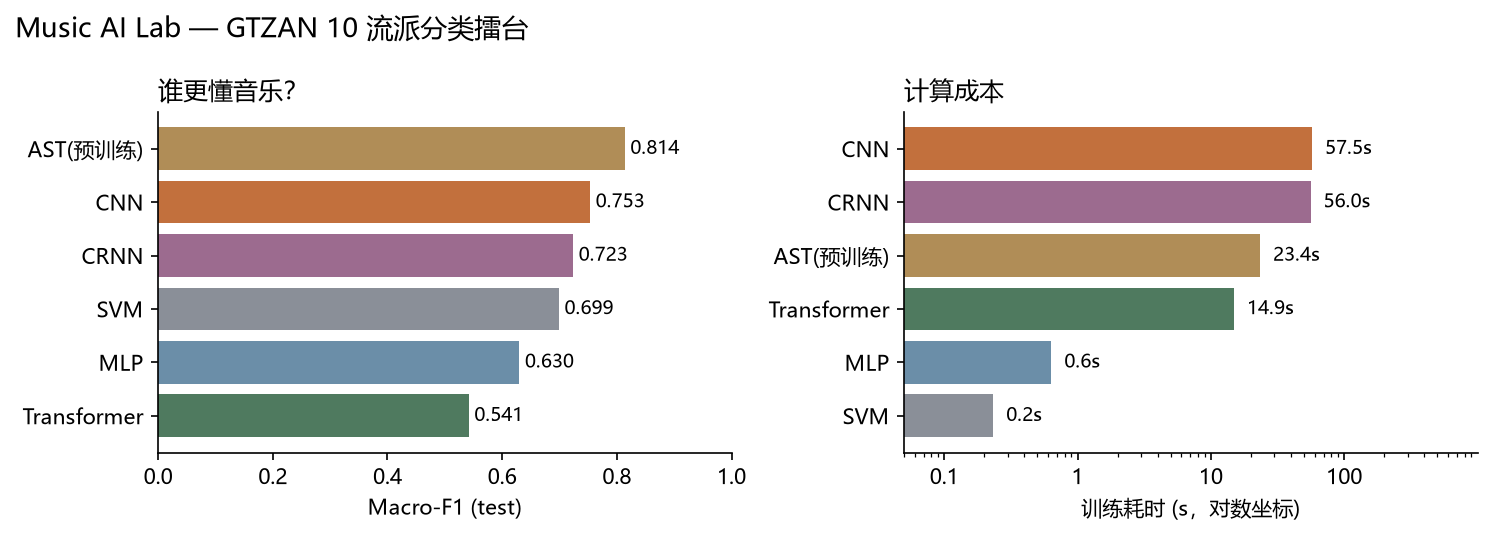
\includegraphics[width=\linewidth]{leaderboard.png}
  \caption{GTZAN 测试集上的 Macro-F1 与训练成本（对数坐标）。AST 为迁移学习组，其训练时间仅含线性头，embedding 提取约 214 s 另计。}
  \label{fig:gtzan-board}
\end{figure}

\begin{figure}[H]
  \centering
  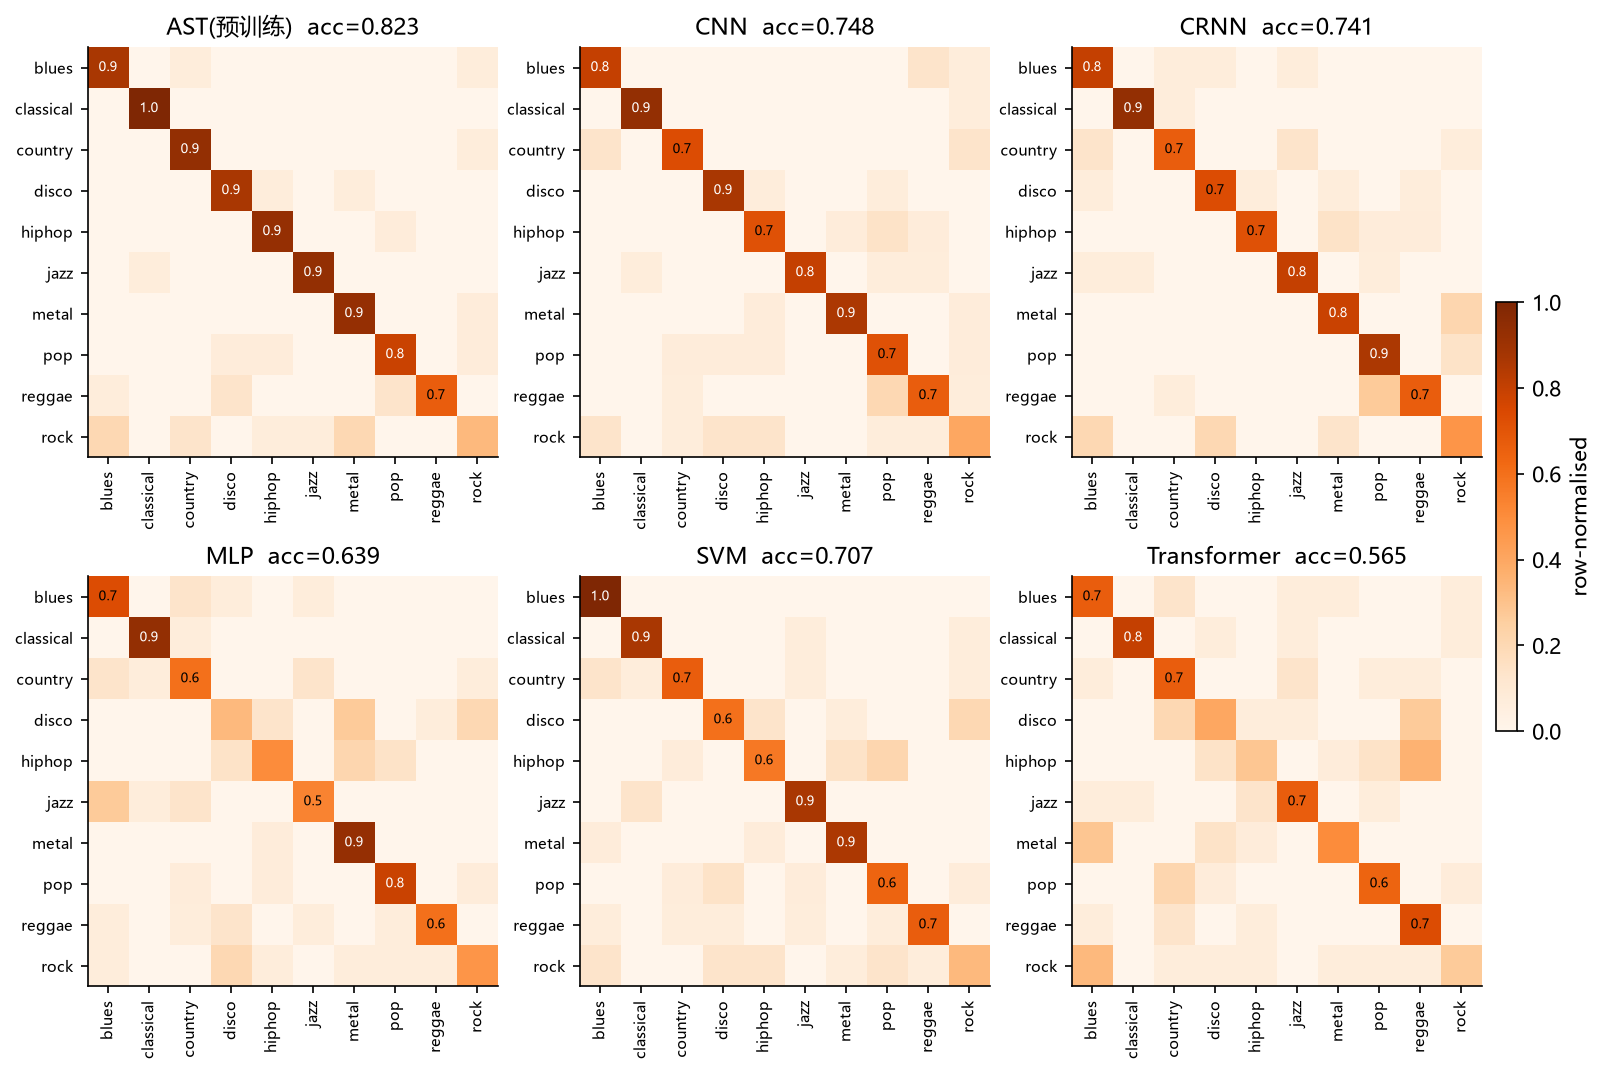
\includegraphics[width=\linewidth]{confusion_matrices.png}
  \caption{GTZAN 测试集混淆矩阵（seed 42，按行归一化）。}
  \label{fig:gtzan-cm}
\end{figure}

\begin{table}[H]
\centering\scriptsize
\caption{GTZAN 逐 seed 结果。}
\label{tab:mvp-perseed}
\begin{tabular}{llcccc}
\toprule
模型 & seed & Acc & Macro-F1 & 训练(s) & 推理(ms)\\
\midrule
ast & 42 & 0.8231 & 0.8135 & 23.4 & 204.06\\
cnn & 42 & 0.7483 & 0.7493 & 57.6 & 0.77\\
cnn & 123 & 0.7551 & 0.7496 & 57.4 & 0.76\\
cnn & 2024 & 0.7619 & 0.7602 & 57.5 & 0.76\\
crnn & 42 & 0.7415 & 0.7411 & 56.3 & 0.76\\
crnn & 123 & 0.6871 & 0.6842 & 55.8 & 0.77\\
crnn & 2024 & 0.7483 & 0.7450 & 55.9 & 0.74\\
mlp & 42 & 0.6395 & 0.6331 & 0.6 & 0.01\\
mlp & 123 & 0.6803 & 0.6825 & 0.4 & 0.01\\
mlp & 2024 & 0.5782 & 0.5735 & 0.9 & 0.04\\
svm & 42 & 0.7075 & 0.6987 & 0.2 & 0.07\\
svm & 123 & 0.7075 & 0.6987 & 0.2 & 0.07\\
svm & 2024 & 0.7075 & 0.6987 & 0.2 & 0.07\\
transformer & 42 & 0.5646 & 0.5566 & 16.6 & 0.27\\
transformer & 123 & 0.5510 & 0.5470 & 17.1 & 0.26\\
transformer & 2024 & 0.5170 & 0.5208 & 11.1 & 0.25\\
\bottomrule
\end{tabular}
\end{table}


从逐 seed 结果可以看到两点：其一，CNN 的三个种子非常稳定（Macro-F1 0.749--0.760，标准差 0.006），说明在小数据上它已经接近自身的容量上限；其二，MLP 与轻量 Transformer 的种子间波动明显更大（MLP 0.574--0.683），这与随机初始化在欠拟合/过拟合边界上的敏感性一致。SVM 的三行完全相同，因为其硬预测与种子无关。

\begin{figure}[H]
  \centering
  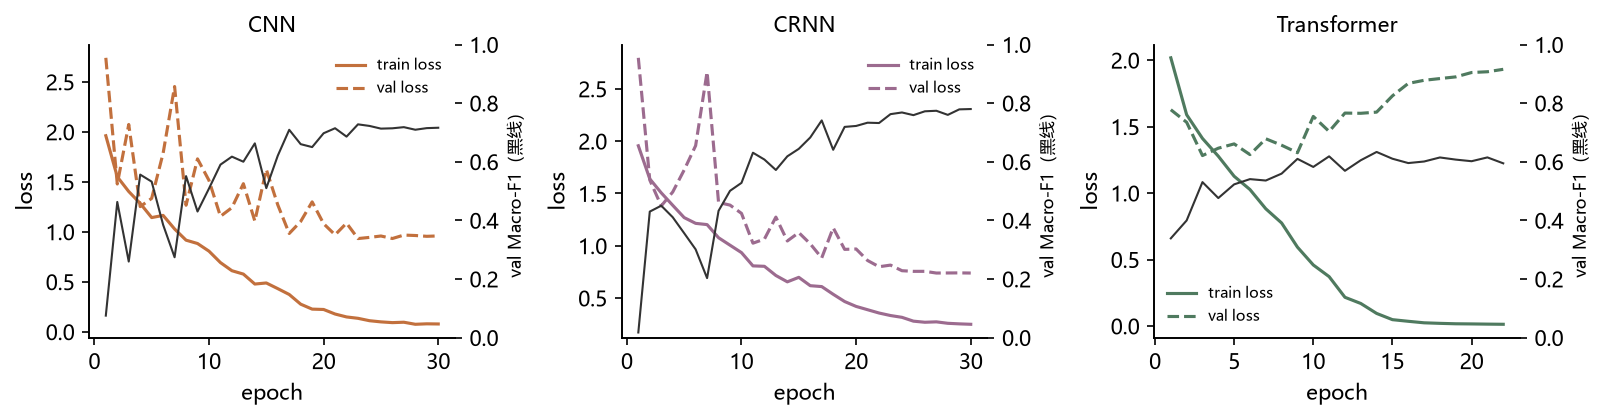
\includegraphics[width=0.95\linewidth]{curves_gtzan.png}
  \caption{GTZAN 上三个深度模型的训练/验证损失与验证 Macro-F1（seed 42）。}
  \label{fig:curves-gtzan}
\end{figure}

训练曲线进一步说明了模型差异：CNN 的验证损失在 20 轮后趋于平稳，CRNN 出现明显振荡，Transformer 的训练损失迅速降到接近 0 而验证损失抬头——这是典型的小样本过拟合。

\subsection{FMA-small：主实验}
表~\ref{tab:fma} 给出 FMA-small 主实验的结果。与 GTZAN 相比，数据规模扩大约 8 倍，测试集约 \FmaTestN{} 首，指标的标准误更小。最佳模型为 \FmaBestModel{}，测试 Macro-F1 为 \FmaBestF{}（Accuracy \FmaBestAcc{}）。在 FMA-small 上，AST（预训练） 取得最高的 Macro-F1（0.590），测试集约 1\,200 首。

\begin{table}[H]
\centering\small
\caption{FMA-small 主实验结果（3 seeds，均值$\pm$标准差；AST 训练时间仅计线性头）。}
\label{tab:fma}
\begin{tabular}{lcccccc}
\toprule
模型 & Acc & Macro-F1 & 训练(s) & 推理(ms) & 参数量 & 大小(MB)\\
\midrule
AST（预训练） & 0.596 & 0.590 & 4.6 & 230.68 & 86.2M & 344.78\\
CNN & 0.480$\pm$0.005 & 0.470$\pm$0.002 & 333.6 & 0.74 & 591K & 2.38\\
CRNN & 0.502$\pm$0.009 & 0.492$\pm$0.006 & 371.3 & 0.76 & 419K & 1.69\\
SVM & 0.446$\pm$0.000 & 0.440$\pm$0.000 & 16.3 & 0.57 & 1.1M & 9.52\\
MLP & 0.428$\pm$0.011 & 0.422$\pm$0.012 & 3.7 & 0.02 & 88K & 1.07\\
Transformer & 0.387$\pm$0.010 & 0.378$\pm$0.019 & 79.8 & 0.26 & 302K & 1.22\\
\bottomrule
\end{tabular}
\end{table}


预训练 AST 的测试 Macro-F1 为 \FmaBestF{}，比最好的自建模型 CRNN（0.492）高约 9.8 个百分点；自建模型中 CRNN 最好，从头训练的 Transformer 只有 0.378，与其在 GTZAN 上的表现一致。AST 的推理延迟约 231 ms/片段、权重 345 MB，约为 CNN 的 300 倍延迟与 145 倍体积。

\begin{figure}[H]
  \centering
  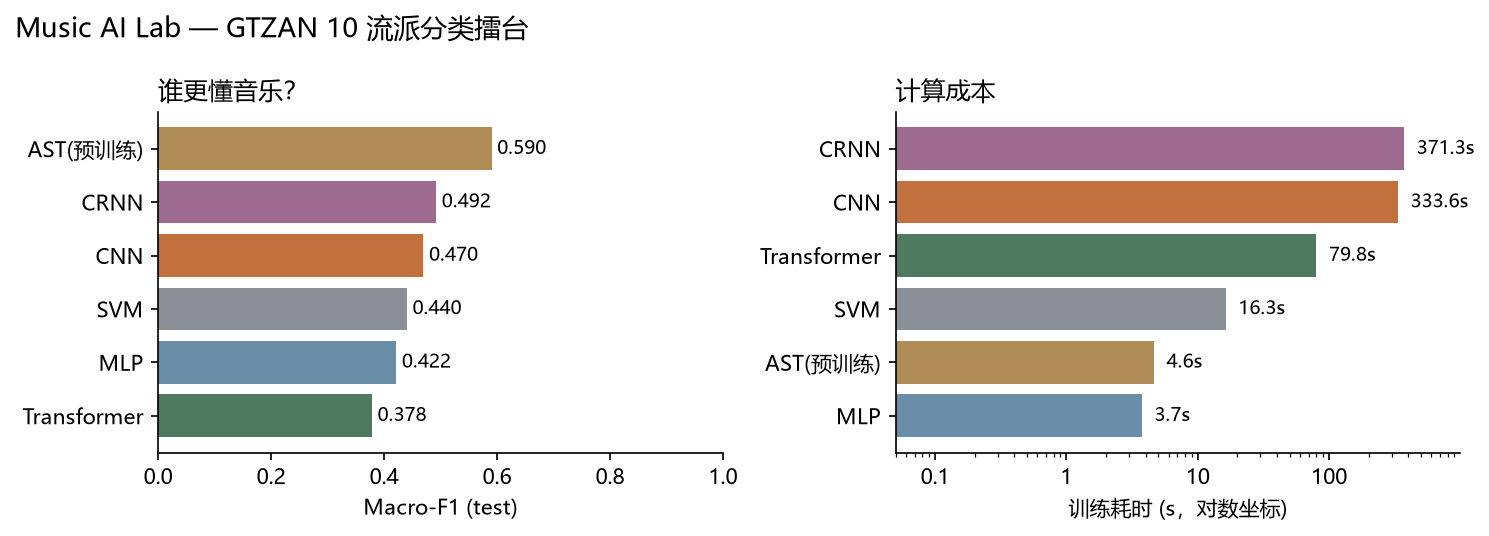
\includegraphics[width=\linewidth]{leaderboard_fma.png}
  \caption{FMA-small 测试集 Macro-F1 与训练成本。AST 的训练时间仅含线性头，约 7 min 的 embedding 提取另计。}
  \label{fig:fma-board}
\end{figure}

\begin{table}[H]
\centering\scriptsize
\caption{FMA-small 逐 seed 结果（AST 为单 seed）。}
\label{tab:fma-perseed}
\begin{tabular}{llcccc}
\toprule
模型 & seed & Acc & Macro-F1 & 训练(s) & 推理(ms)\\
\midrule
ast & 42 & 0.5963 & 0.5903 & 4.6 & 230.68\\
cnn & 42 & 0.4746 & 0.4712 & 314.2 & 0.71\\
cnn & 123 & 0.4804 & 0.4701 & 328.5 & 0.74\\
cnn & 2024 & 0.4862 & 0.4675 & 357.9 & 0.76\\
crnn & 42 & 0.4912 & 0.4871 & 451.5 & 0.80\\
crnn & 123 & 0.5138 & 0.5006 & 390.7 & 0.73\\
crnn & 2024 & 0.5013 & 0.4886 & 271.5 & 0.75\\
mlp & 42 & 0.4429 & 0.4377 & 4.0 & 0.01\\
mlp & 123 & 0.4204 & 0.4169 & 3.8 & 0.01\\
mlp & 2024 & 0.4195 & 0.4101 & 3.5 & 0.02\\
svm & 42 & 0.4462 & 0.4404 & 16.1 & 0.56\\
svm & 123 & 0.4462 & 0.4404 & 16.3 & 0.63\\
svm & 2024 & 0.4462 & 0.4404 & 16.4 & 0.53\\
transformer & 42 & 0.3928 & 0.3974 & 77.5 & 0.25\\
transformer & 123 & 0.3728 & 0.3524 & 78.3 & 0.27\\
transformer & 2024 & 0.3953 & 0.3855 & 83.6 & 0.25\\
\bottomrule
\end{tabular}
\end{table}


\begin{table}[H]
\centering\small
\caption{FMA-small 逐类 F1（seed 42）与测试样本数。}
\label{tab:fma-perclass}
\begin{tabular}{lcccc}
\toprule
流派 & CNN & CRNN & AST & 测试样本\\
\midrule
Electronic & 0.590 & 0.539 & 0.679 & 139\\
Experimental & 0.438 & 0.465 & 0.489 & 147\\
Folk & 0.447 & 0.511 & 0.577 & 137\\
Hip-Hop & 0.674 & 0.671 & 0.797 & 135\\
Instrumental & 0.258 & 0.281 & 0.366 & 126\\
International & 0.507 & 0.563 & 0.669 & 156\\
Pop & 0.239 & 0.258 & 0.430 & 191\\
Rock & 0.617 & 0.608 & 0.715 & 168\\
\bottomrule
\end{tabular}
\end{table}


\begin{figure}[H]
  \centering
  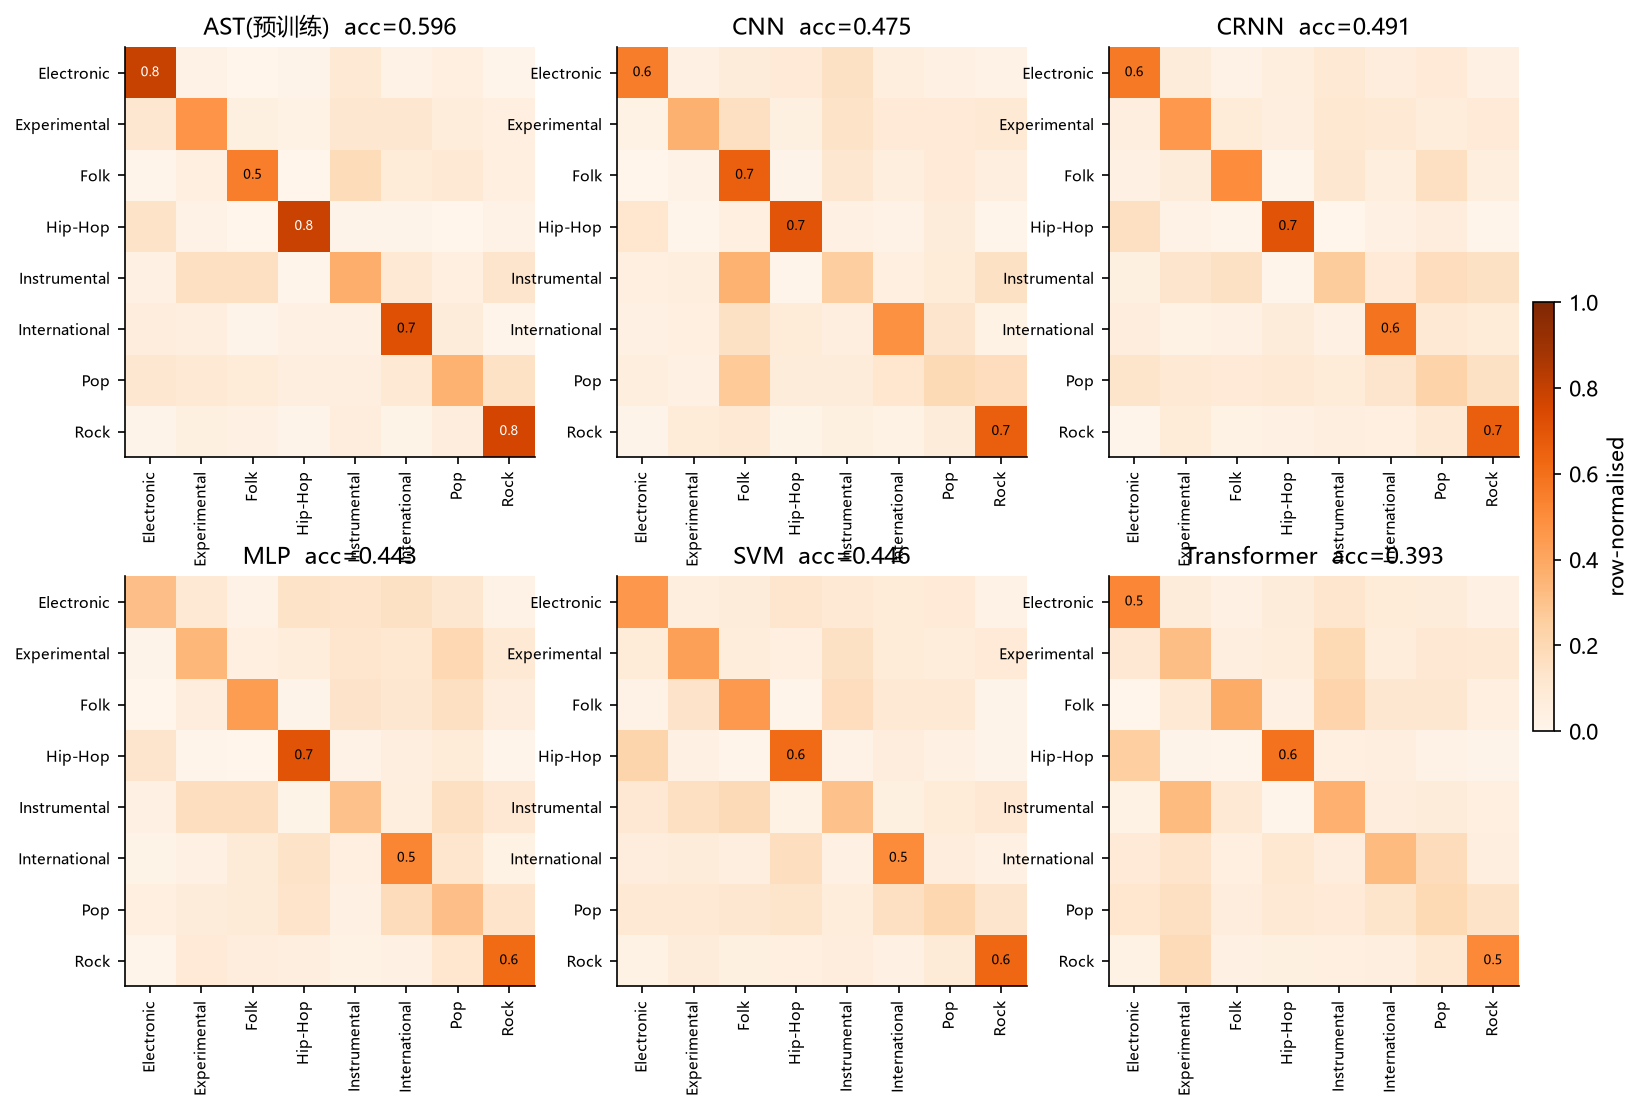
\includegraphics[width=0.98\linewidth]{confusion_fma.png}
  \caption{FMA-small 测试集混淆矩阵（seed 42，按行归一化），六个模型对比。}
  \label{fig:fma-cm}
\end{figure}

\begin{figure}[H]
  \centering
  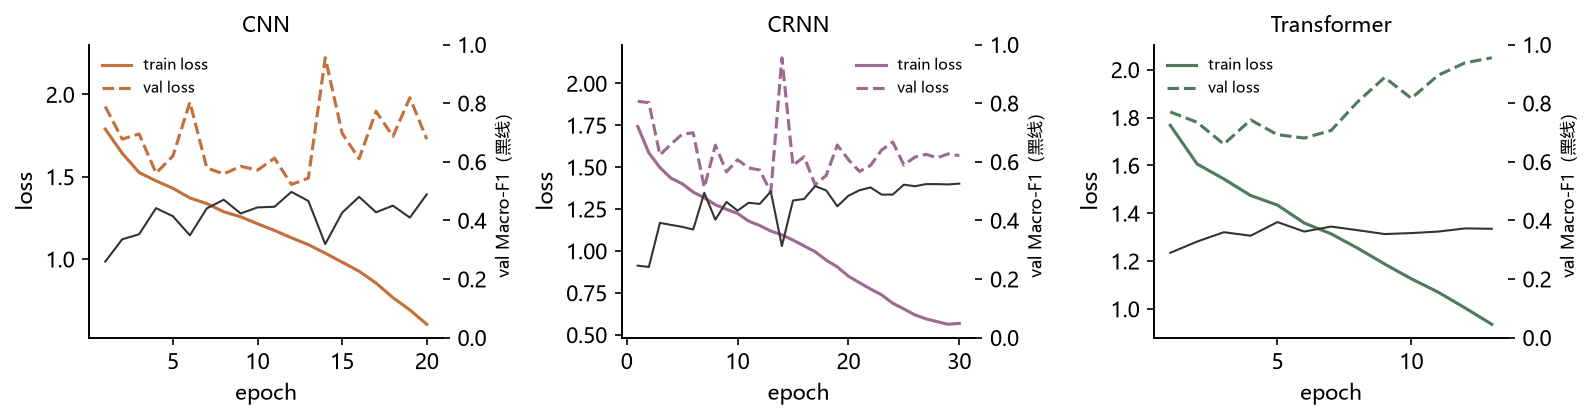
\includegraphics[width=0.95\linewidth]{curves_fma.png}
  \caption{FMA-small 上 CNN / CRNN / Transformer 的训练曲线（seed 42）。}
  \label{fig:curves-fma}
\end{figure}

逐类结果揭示了 FMA 的难点：CNN 在 Pop（F1 0.239）与 Instrumental（0.258）上最差，
在 Hip-Hop（0.674）与 Rock（0.617）上最好；AST 把 Pop 提升到 0.430、Instrumental 提升到
0.366，但依然远低于其余类别。这说明「Pop」「Instrumental」这类宽标签本身覆盖了多种风格，
单一片段、单一标签的监督信号不足以区分。

为量化「按曲目划分」的泄漏影响，我们用同一批特征、仅把划分换成曲目级（测试集与训练集共享艺术家的比例为 81.0\%），重新训练 CNN。曲目级划分下 CNN 的测试 Macro-F1 为 \LeakCnnF{}（Acc \LeakCnnAcc{}），相比艺术家分离划分的 \FmaCnnF{} 变化 \LeakDelta{} 个百分点。这一差异说明：\textbf{在 FMA 这类元数据完整的语料上，不按艺术家划分会系统性地高估模型能力}；因此本文主表全部采用艺术家分离结果。

\subsection{优化消融}
表~\ref{tab:ablation} 比较了基线、SpecAugment、SpecAugment+标签平滑三种配置（seed 42，20 epoch，仅验证集，测试集不参与选型）。验证集上最佳配置为 CNN + SpecAug + LS（Macro-F1 0.529），但相对 CNN 基线仅提升 +0.7 个百分点，处于单次运行的波动范围内；因此主实验保留基线配置，不引入额外复杂度。 这一负结果本身有信息量：FMA 上的主要瓶颈不是「模型记住训练集」，而是\textbf{流派标签边界模糊与音乐多样性}——正则化能让训练/验证损失更接近，却无法凭空提供可区分的声学线索。

\begin{table}[H]
\centering\small
\caption{优化消融（FMA-small 验证集，seed 42，20 epoch；测试集未参与选型）。}
\label{tab:ablation}
\begin{tabular}{lccc}
\toprule
配置 & val Acc & val Macro-F1 & best epoch\\
\midrule
CNN baseline & 0.542 & 0.522 & 17\\
CNN + SpecAug & 0.540 & 0.520 & 16\\
CNN + SpecAug + LS & 0.554 & 0.529 & 16\\
CRNN + SpecAug + LS & 0.560 & 0.524 & 20\\
Transformer + SpecAug + LS & 0.422 & 0.394 & 20\\
\bottomrule
\end{tabular}
\end{table}


\subsection{训练预算消融}\label{sec:budget}

上文的全部结果都建立在固定预算上（30 轮、早停 patience 8）。事后复核发现，
部分模型的最优轮次正好落在这个上限上（GTZAN 的 CNN seed 123 与 CRNN seed 42、
FMA 的 CRNN seed 42 均为第 30 轮），因此有必要检验「继续训练是否还会更好」。
我们把两个数据集的三个深度模型统一加长到 60 轮、patience 12，其余协议完全不变，
结果见表~\ref{tab:budget}。\BudgetSentence

\begin{table}[H]
\centering\small
\caption{训练预算消融：原协议（30 轮，patience 8）与加长（60 轮，patience 12）的测试集 Macro-F1 对比。所有配置沿用同一数据划分与随机种子。}
\label{tab:budget}
\begin{tabular}{llccc}
\toprule
数据集 & 模型 & 原预算 & 加长训练 & $\Delta$\\
\midrule
GTZAN & CNN & 0.7530 & 0.7606 & $+0.0075$\\
 & CRNN & 0.7234 & 0.7370 & $+0.0136$\\
 & 轻量 Transformer & 0.5415 & 0.5348 & $-0.0067$\\
\midrule
FMA-small & CNN & 0.4696 & 0.4611 & $-0.0085$\\
 & CRNN & 0.4921 & 0.4844 & $-0.0077$\\
 & 轻量 Transformer & 0.3784 & 0.3808 & $+0.0024$\\
\bottomrule
\end{tabular}
\end{table}


这个结果有两个含义。其一，\textbf{主实验的训练预算基本是充分的}：
FMA 上三个模型要么持平要么略微下降，说明早停并没有系统性地截断仍在改善的模型，
原结果不需要因为「没训够」而打折扣。其二，\textbf{小数据集上的方差不容忽视}：
GTZAN 测试集只有 147 首，CNN 的 $+0.75$ 与 CRNN 的 $+1.36$ 个百分点在单一种子下
很难与随机波动区分；而轻量 Transformer 加长后反而更差，与它在 GTZAN 上早已
明显过拟合（最优轮次在第 7--13 轮就出现）的判断一致。
我们因此\textbf{不把表~\ref{tab:budget} 的小幅提升替换进主表}，而是作为稳健性检查保留。

\subsection{计算成本与部署取舍}

表~\ref{tab:cost} 汇总了部署相关的指标。自建模型的权重大小在 1--2.4\,MB、单片段延迟低于
1\,ms，适合浏览器端或嵌入式部署；AST 的权重为 345\,MB、延迟约 231\,ms，更适合离线批量标注。
需要指出，AST 的 4.6\,s「训练时间」只是线性头，8,000 首的 embedding 提取约需 7 分钟（12 进程
特征化 + fp16 GPU 前向），这部分成本在迁移学习中不可忽略。

\begin{table}[H]
\centering\small
\caption{部署相关指标对比（GTZAN / FMA 两套权重结构相同）。}
\label{tab:cost}
\begin{tabular}{lcccc}
\toprule
模型 & 参数量 & 大小 (MB) & 推理 (ms/片段) & 训练成本\\
\midrule
MLP & 87,946 & 1.07 & 0.02 & 0.6\,s\\
SVM & 140,657 & 1.23 & 0.07 & 0.2\,s\\
Transformer & 302,474 & 1.22 & 0.26 & 15\,s\\
CRNN & 418,986 & 1.69 & 0.76 & 55\,s\\
CNN & 592,554 & 2.39 & 0.76 & 57\,s\\
AST（冻结） & 86,194,954 & 346.45 & 204--231 & 23\,s + 提取\\
\bottomrule
\end{tabular}
\end{table}

% ================= 7 分析 =================
\subsection{错误分析}
在 GTZAN 上，CNN 最常见的混淆对是 \texttt{reggae}$\rightarrow$\texttt{pop}、\texttt{blues}$\rightarrow$\texttt{reggae} 与 \texttt{hiphop}$\rightarrow$\texttt{pop}；\texttt{rock} 的逐类 F1 最低（0.429），\texttt{classical} 最高（0.933）。置信度并不等于正确率：Transformer 的 64 个错误中有 16 个置信度超过 0.9，而 CNN 只有 3/37。在 FMA 主实验上，CNN 的错误更分散（Pop$\rightarrow$Folk 52 首、Instrumental$\rightarrow$Folk 45 首、Pop$\rightarrow$Rock 33 首），CRNN 的高置信错误为 90/610，远高于 CNN 的 23/630。这说明模型在标签边界模糊的样本上会「自信地犯错」，现场演示时比单纯报准确率更有说服力。

\begin{table}[H]
\centering\small
\caption{GTZAN 逐类 F1（seed 42）：CNN 与预训练 AST 对比。}
\label{tab:perclass}
\begin{tabular}{lccc}
\toprule
流派 & CNN F1 & AST F1 & 测试样本\\
\midrule
rock & 0.429 & 0.417 & 15\\
pop & 0.625 & 0.786 & 15\\
reggae & 0.667 & 0.800 & 15\\
hiphop & 0.690 & 0.867 & 15\\
country & 0.759 & 0.875 & 15\\
blues & 0.774 & 0.812 & 15\\
disco & 0.839 & 0.839 & 15\\
jazz & 0.889 & 0.933 & 15\\
metal & 0.889 & 0.839 & 15\\
classical & 0.933 & 0.968 & 15\\
\bottomrule
\end{tabular}
\end{table}


\begin{figure}[H]
  \centering
  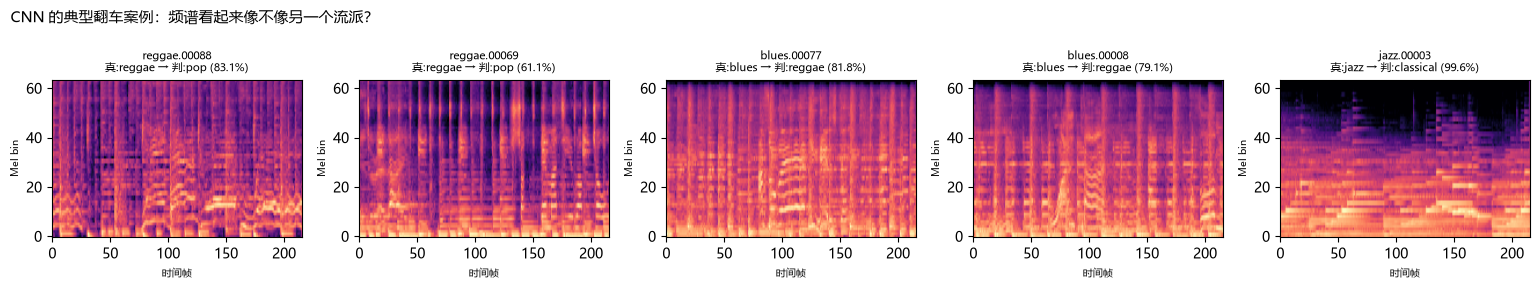
\includegraphics[width=\linewidth]{error_cases.png}
  \caption{CNN 典型错误案例的 Log-Mel 对照（真值 $\rightarrow$ 预测，括号为置信度）。}
  \label{fig:error-cases}
\end{figure}

\subsection{鲁棒性}
表~\ref{tab:robust} 与图~\ref{fig:robust} 汇总 5 个模型在 7 种扰动下的测试准确率（GTZAN，seed 42）。三个现象值得强调：
（1）深度模型对整体增益\textbf{完全不变}，因为 Log-Mel 以片段最大值为参考；SVM/MLP 因使用绝对 dB 的 MFCC 与 RMS 而掉 0.7--3.4 个百分点。
（2）噪声破坏最大，10\,dB SNR 下平均掉约 42 个百分点，0\,dB 时 CNN 从第一名变成最差（0.122）。
（3）除增益外，每个扰动条件下绝对准确率第一都是 SVM——深度模型赢在干净输入，传统模型赢在输入变脏时。

\begin{table}[H]
\centering\small
\caption{七种扰动下的测试准确率（GTZAN，seed 42，n=147）。}
\label{tab:robust}
\begin{tabular}{lccccccc}
\toprule
模型 & clean & 3s & 10s & 0.5$\times$ & 1.5$\times$ & 10dB & 0dB\\
\midrule
SVM & 0.708 & 0.578 & 0.748 & 0.701 & 0.673 & 0.333 & 0.299\\
MLP & 0.639 & 0.531 & 0.701 & 0.612 & 0.633 & 0.272 & 0.218\\
CNN & 0.748 & 0.408 & 0.537 & 0.748 & 0.748 & 0.211 & 0.122\\
CRNN & 0.742 & 0.211 & 0.524 & 0.742 & 0.742 & 0.252 & 0.163\\
Transformer & 0.565 & 0.531 & 0.599 & 0.565 & 0.565 & 0.231 & 0.150\\
\bottomrule
\end{tabular}
\end{table}


\begin{figure}[H]
  \centering
  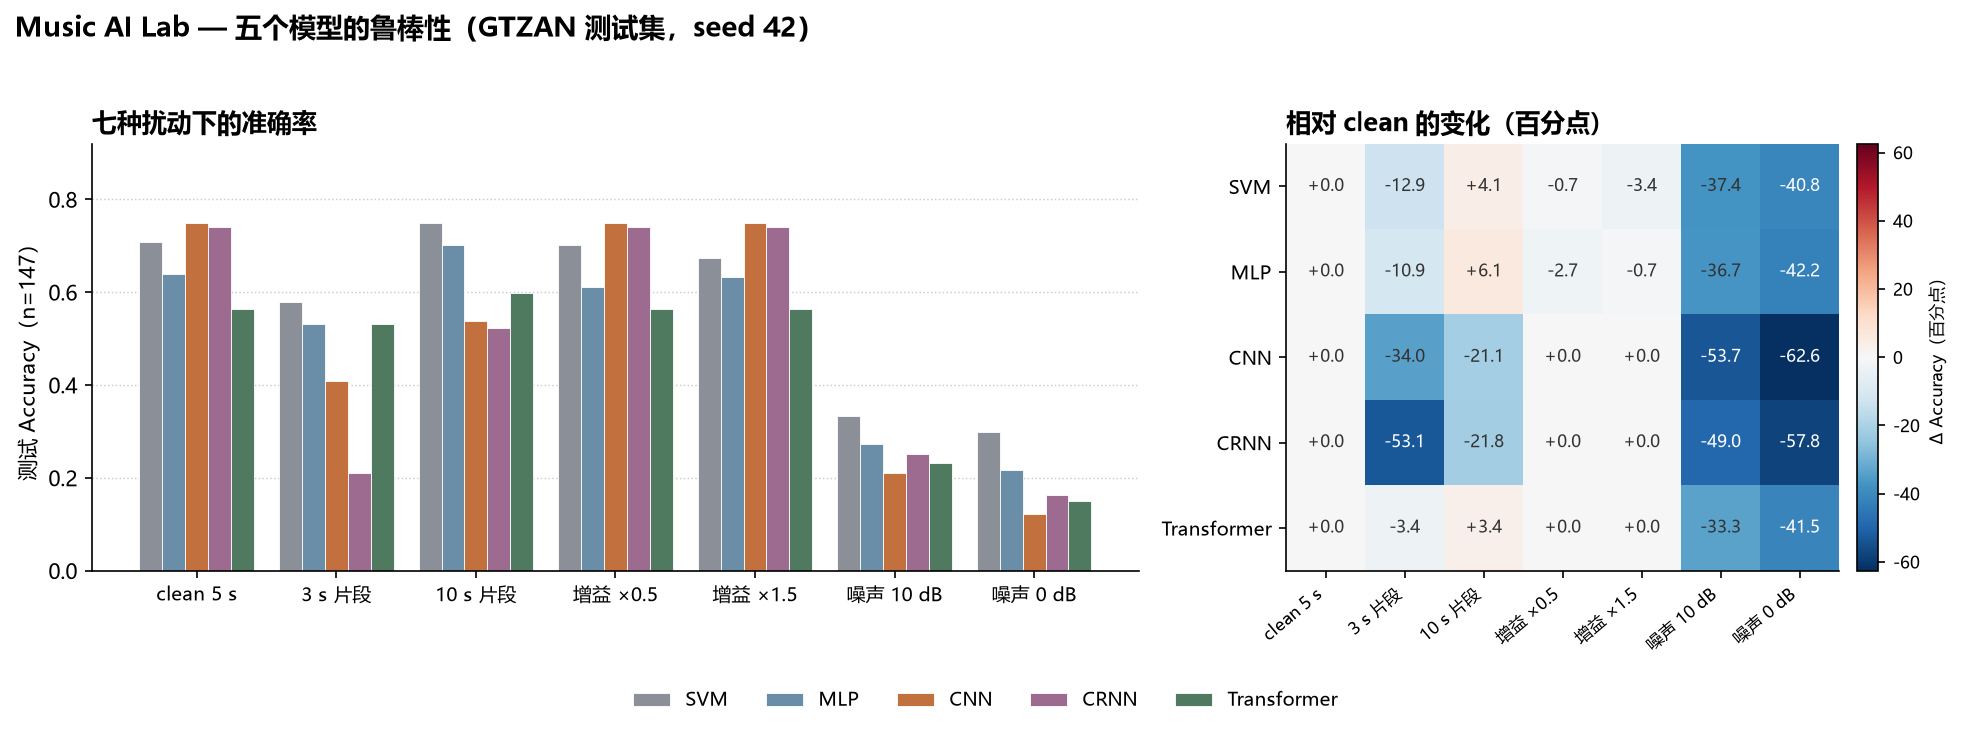
\includegraphics[width=\linewidth]{robustness.png}
  \caption{七种扰动下的准确率与相对 clean 的变化（百分点）。}
  \label{fig:robust}
\end{figure}

\subsection{片段级分析}
把一首歌切成 5 秒窗口、步长 2.5 秒逐段预测，147 首测试曲目中有 88 首至少出现一次判断变化。\texttt{rock.00072} 在 11 个窗口中改判 9 次，而 classical 曲目全程稳定。这说明流派不是整首歌的静态标签，也提示片段长度会直接影响模型输入的信息量。

\begin{figure}[H]
  \centering
  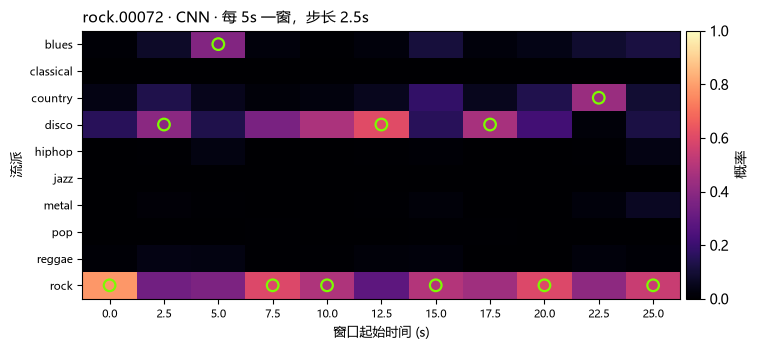
\includegraphics[width=0.92\linewidth]{timeline_rock.00072.png}
  \caption{\texttt{rock.00072} 的滑动窗口预测时间轴（绿圈为各窗口 Top-1）。}
  \label{fig:timeline}
\end{figure}

\projectpart{II\quad 生成式任务：离散 Token 预测与音频续写}
\section[二期：离散 Token 预测与音乐生成]{二期扩展：从判别式分类到离散 Token 预测与音乐生成}\label{sec:phase2}

一期的全部实验都是判别式的：给定 5 秒音频，输出 10 个（或 8 个）流派标签之一。
一个自然的问题是——同一个系统能否回答"接下来会发生什么"？本章把任务从"分类"
推进到"预测"与"生成"，并严格区分两类结果：一是对\textbf{真实未来}的 Token 级预测，
二是在\textbf{前缀条件}下的音乐续写。前者可以用交叉熵和 Top-1 精确度量，后者只能部分
度量、必须结合试听，二者的评价口径不能混用。

\subsection{任务定义与动机}\label{sec:p2motivation}

一期与二期的差别可以写成两个不同的条件分布：

\begin{itemize}
  \item 分类：$p(y \mid \mathbf{x}_{1:T})$，$y$ 为流派标签，$\mathbf{x}$ 为 5 秒音频；
  \item 预测：$p(\mathbf{c}_{T+1:T+K} \mid \mathbf{c}_{1:T})$，$\mathbf{c}$ 为离散音频 Token；
  \item 生成：$p(\mathbf{x}_{T+1:T+K'} \mid \mathbf{x}_{1:T}, \text{text})$，输出是可播放的波形。
\end{itemize}

选择 Token 而不是波形，有两个工程理由。第一，离散 Token 把"预测音频"变成了
"预测离散符号"，可以直接复用语言模型的训练与评价方法（交叉熵、Top-$k$、自回归
roll-out），不需要设计波形回归损失或对抗训练。第二，它把"模型是否学到了音乐的
时间结构"与"声码器是否好听"解耦——若 Token 预测很差，问题就不在解码器。

本章的实验设计刻意保持"可控"：Token 预测部分只用 5 秒前缀预测 1 秒真实未来，
模型是自己训练的小网络，不调用任何生成大模型；生成部分才引入预训练的
MusicGen-small，并先验证原始模型能跑通、再讨论轻量适配。

\subsection{离散音频 Token：EnCodec 32 kHz}\label{sec:encodec}

编码器选用 \texttt{facebook/encodec\_32khz}，即 MusicGen 使用的同款配置。它把
32 kHz 单声道波形经卷积编码器与残差向量量化（RVQ）压成 4 个码本、每码本 2048 个
词条的离散序列，帧率 50 Hz，目标带宽 2.2 kbps。表~\ref{tab:encodec} 给出实测规格。

\begin{table}[H]
\centering\small
\caption{EnCodec 32 kHz 的实测规格（6 秒窗口）。}\label{tab:encodec}
\begin{tabular}{ll}
\toprule
项目 & 实测值\\
\midrule
检查点 / 参数量 & \texttt{facebook/encodec\_32khz} / 56.9\,M（约 228\,MB）\\
采样率 / 声道 & 32\,000\,Hz / 单声道\\
码本数与词表 & 4 个码本 $\times$ 2\,048\\
帧率 & 50\,Hz（1\,s $=$ 50 帧，6\,s $=$ 300 帧）\\
6 秒窗口 Token 量 & $4 \times 300 = 1\,200$\\
编码输出形状 & \texttt{audio\_codes} $=(n_{\text{frames}},\,B,\,4,\,T)$，本实验 $n_{\text{frames}}=1$\\
解码回波形 & \texttt{audio\_values} $=(B,\,T\times 640)$，48\,k 采样点 $=$ 6\,s\\
编码吞吐（8 卡批次） & 8$\times$6\,s 约 0.34\,s（fp32，RTX 4060）\\
\bottomrule
\end{tabular}
\end{table}

有一个容易被忽略的兼容性细节：\texttt{transformers} 的编码输出第一维是
"分段数"而不是批大小，若直接把 \texttt{audio\_codes[:, 0]} 当作批维，
批内除第一段以外的样本会被静默丢弃——本项目在第一次全量编码时就踩了这个坑
（每 512 个窗口只写入 1 行 Token），发现后修正并重跑。这类"形状对得上、语义却错"
的 bug 不会报错，只会让数据静默变少，因此下表的所有统计都同时核对了 Token 行数与
窗口行数。

\subsection{数据窗口与泄漏控制}\label{sec:p2data}

数据沿用 FMA-small 与一期按艺术家分离的划分（5\,596 / 1\,199 / 1\,199）。
每首曲目在其内部取 2 个不重叠的 6 秒窗口：前 5 秒作为前缀（250 帧），
后 1 秒作为预测目标（50 帧）。窗口继承曲目所属划分，因此\textbf{同一首歌的窗口不会同时出现在训练集与测试集}——这正是分类实验里那条"按艺术家划分"的约束在预测任务
上的对应物。最终得到 \TokNTrain{} 个训练窗口、测试集 \TokNTest{} 个窗口
（\TokNTracks{} 首曲目），Token 缓存以 shard 形式落盘，编码中断可从断点续跑。

\subsection{预测模型}\label{sec:p2models}

所有模型都做同一件事：给定前 $t$ 帧的 4 个码本，预测第 $t+1$ 帧的 4 个码本。
四条流共享一个主干，输出 4 个独立分类头（MusicGen 式的并行码本预测），
这样可以避免自回归解码时四条流不同步的问题。

\begin{table}[H]
\centering\small
\caption{Token 预测模型与基线。}\label{tab:tokenmodels}
\begin{tabular}{l p{7.6cm} r}
\toprule
模型 & 结构 & 参数量\\
\midrule
Persistence & 重复前缀最后一帧，不做任何学习 & 0\\
频率先验 & 训练集各码本最高频 Token & 0\\
Bigram & $p(t\mid t-1)$ 加 0.5 平滑，回落至 unigram & 0\\
LSTM & 4 个 Embedding 求和 $+$ 位置编码 $+$ 2 层 LSTM(256) $+$ 4 头 & 5.3\,M\\
Transformer & 4 个 Embedding 求和 $+$ 位置编码 $+$ 4 层因果注意力($d=192$, 4 头) $+$ 4 头 & \TokTfParams\\
\bottomrule
\end{tabular}
\end{table}

选择"并行码本"而不是"逐码本级联"，代价是模型必须同时刻画四条残差流之间的
相关性；收益是推理时一次前向就能得到完整的一帧，且解码器可以直接消费。
单码本（只预测码本 0）是更便宜的简化，但它\textbf{无法单独解码}，因此本文不做单码本
主结果，只把它作为反面对照写进局限性。

\subsection{训练与评价口径}\label{sec:p2train}

训练目标是四个码本的平均交叉熵。优化器 AdamW（学习率 $3\times10^{-4}$，权重衰减
0.01），余弦退火，梯度裁剪 1.0，batch 64，早停耐心 3 个 epoch，按验证集 NLL 选择
最优权重；每个模型跑 3 个随机种子（42/123/2024），测试集只在最后评估一次。

评价分两种口径，必须同时报告：

\begin{itemize}
  \item \textbf{teacher-forced}：第 $t$ 步喂入真实的历史 Token，度量"给定正确历史时
        分布有多准"，即标准的 NLL / Top-1；
  \item \textbf{free-running}：模型把自己的预测喂回下一步，度量"真正生成时"的准确率。
        两者差距越大，说明误差累积越严重。
\end{itemize}

\subsection{Token 预测结果}\label{sec:p2results}

\begin{table}[H]
\centering\small
\caption{Token 预测结果（FMA-small 测试集，5 s 前缀 → 1 s 目标）。神经网络为 3 个种子的均值 $\pm$ 标准差，基线为确定性预测。}
\label{tab:token}
\begin{tabular}{lccccc}
\toprule
模型 & 参数量 & NLL & Teacher Top-1 & Free Top-1 & 码本 0 Top-1\\
\midrule
Persistence & -- & -- & 0.016 & 0.016 & 0.024\\
频率先验 & -- & -- & 0.012 & 0.012 & 0.009\\
Bigram & -- & -- & 0.017 & 0.017 & 0.024\\
LSTM & 5.3M & 6.821 & 0.020$\pm$0.000 & 0.016$\pm$0.000 & 0.016\\
Transformer & 5.0M & 6.725 & 0.024$\pm$0.000 & 0.019$\pm$0.000 & 0.023\\
\bottomrule
\end{tabular}
\end{table}


\begin{figure}[H]
\centering
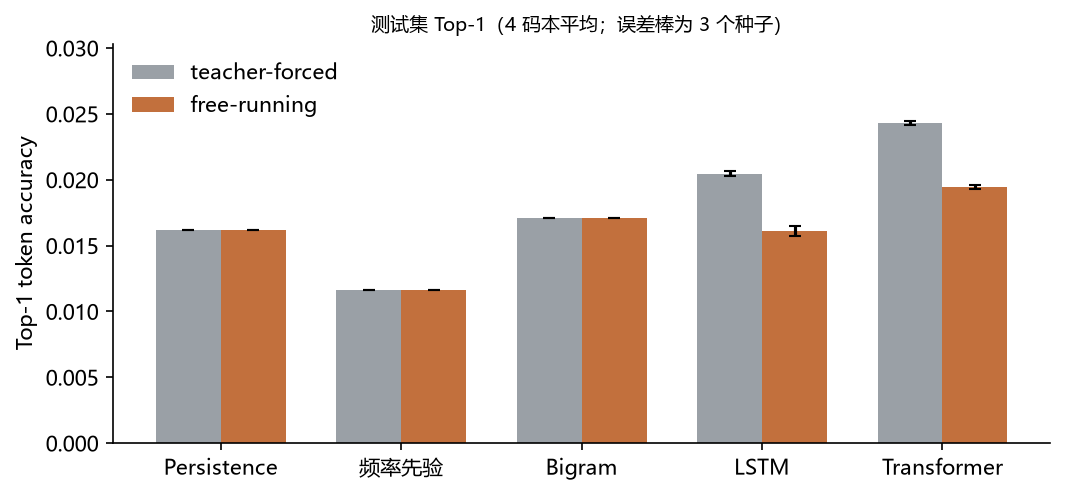
\includegraphics[width=\textwidth]{token_top1.png}
\caption{测试集 Top-1（4 码本平均）。灰色为 teacher-forced，橙色为 free-running，
误差棒为 3 个种子的标准差。}\label{fig:tokentop1}
\end{figure}

\begin{figure}[H]
\centering
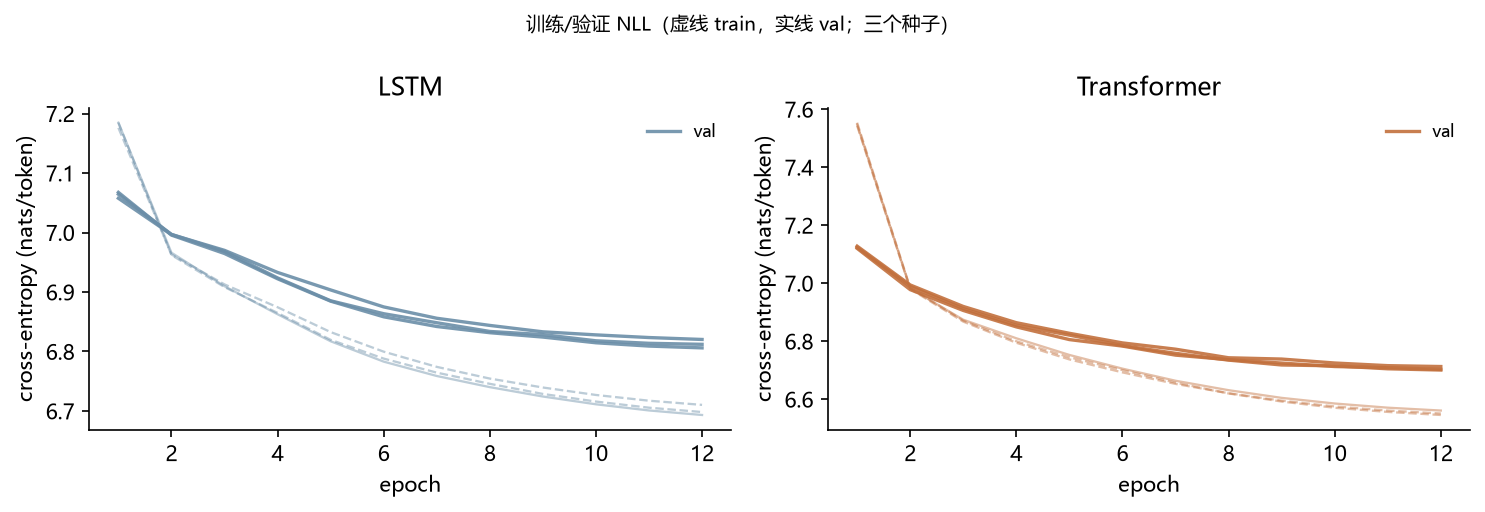
\includegraphics[width=0.92\textwidth]{token_curves.png}
\caption{训练与验证 NLL 曲线：三个种子的验证曲线几乎重合，说明小模型在固定数据上
训练稳定。}\label{fig:tokencurves}
\end{figure}

\begin{figure}[H]
\centering
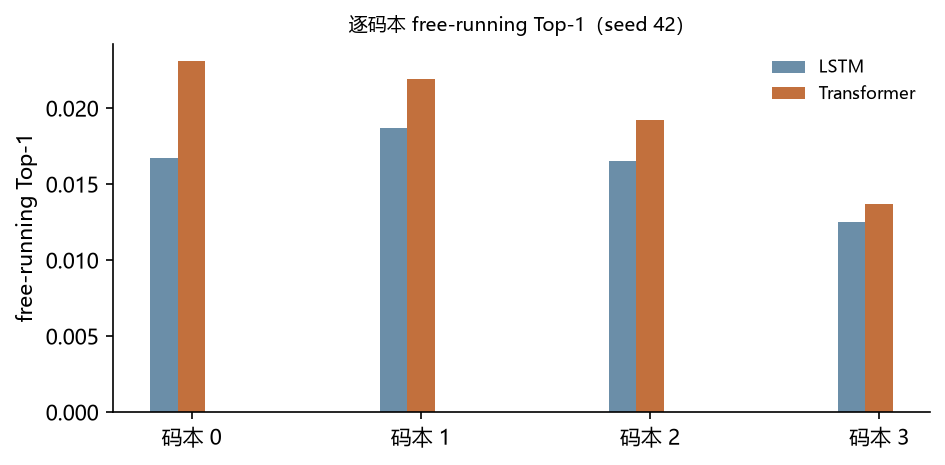
\includegraphics[width=0.78\textwidth]{token_per_codebook.png}
\caption{逐码本 free-running Top-1（seed 42）。码本 0 最容易，靠后的残差码本更难，
与 RVQ 的残差结构一致。}\label{fig:tokencb}
\end{figure}

四点观察：

\begin{enumerate}
  \item \textbf{学习信号真实存在，但绝对水平很低。}随机猜的 Top-1 是 $1/2048=0.049\%$；
        Transformer 的 free-running Top-1 为 \TokTransformerFree{}，约为随机的 40 倍，
        比最好的统计基线 Bigram（\TokBigramFree{}）高 0.24 个百分点（相对提升约 14\%）；
        NLL 从均匀分布的值 $\ln 2048 = 7.62$ 降到 \TokTransformerNll{}。
  \item \textbf{误差累积是主要损失来源。}Transformer 的 teacher-forced Top-1 为
        \TokTfTeacher{}，free-running 掉到 \TokTransformerFree{}；LSTM 也从
        \TokLstmFree{} 的教师强制口径下降。一旦让模型吃自己的预测，错误逐步放大——
        这正是自回归模型在长 horizon 上的典型退化。
  \item \textbf{LSTM 没有赢过 n-gram。}LSTM 的 free-running Top-1（\TokLstmFree{}）甚至
        略低于 Bigram（\TokBigramFree{}）。原因不是"没训练好"（其 NLL 明显低于 Bigram），
        而是循环状态在自回归回灌下更不稳定；小 Transformer 的因果注意力在本任务上更有效。
  \item \textbf{第一码本靠"重复"就够，增益来自残差码本。}Persistence 在码本 0 上能拿到
        2.43\%，与 Transformer 的 2.31\% 相当；但四码本平均时 Persistence 只有
        \TokPersistenceFree{}。这说明码本 0 高度局部平滑（音乐瞬时音色变化慢），
        神经模型的收益主要来自后三个残差码本。
\end{enumerate}

\subsection{把 Token 解码回音频}\label{sec:p2decode}

预测得准不等于"能听"。由于本实验预测全部 4 个码本，可以直接交给 EnCodec 解码：

\begin{enumerate}
  \item 用模型自回归生成 50 帧 $\times$ 4 码本；
  \item 送入 EnCodec 解码器得到 1 秒波形；
  \item 与原曲真实后 1 秒做 Log-Mel 对照，并保存 wav 供试听。
\end{enumerate}

\begin{table}[H]
\centering\small
\caption{预测 Token 解码回音频后与真实后 1 秒的对照（Log-Mel RMSE，越小越接近）。}
\label{tab:tokensamples}
\begin{tabular}{llcc}
\toprule
曲目 & 流派 & Log-Mel RMSE & 试听\\
\midrule
001482 & Electronic & 14.43 & \texttt{001482\_Electronic\_pred.wav}\\
000995 & Experimental & 7.74 & \texttt{000995\_Experimental\_pred.wav}\\
000814 & Folk & 13.73 & \texttt{000814\_Folk\_pred.wav}\\
007481 & Hip-Hop & 18.01 & \texttt{007481\_Hip-Hop\_pred.wav}\\
014568 & Instrumental & 21.13 & \texttt{014568\_Instrumental\_pred.wav}\\
000704 & International & 17.05 & \texttt{000704\_International\_pred.wav}\\
000010 & Pop & 13.12 & \texttt{000010\_Pop\_pred.wav}\\
000182 & Rock & 15.33 & \texttt{000182\_Rock\_pred.wav}\\
\bottomrule
\end{tabular}
\end{table}


\begin{figure}[H]
\centering
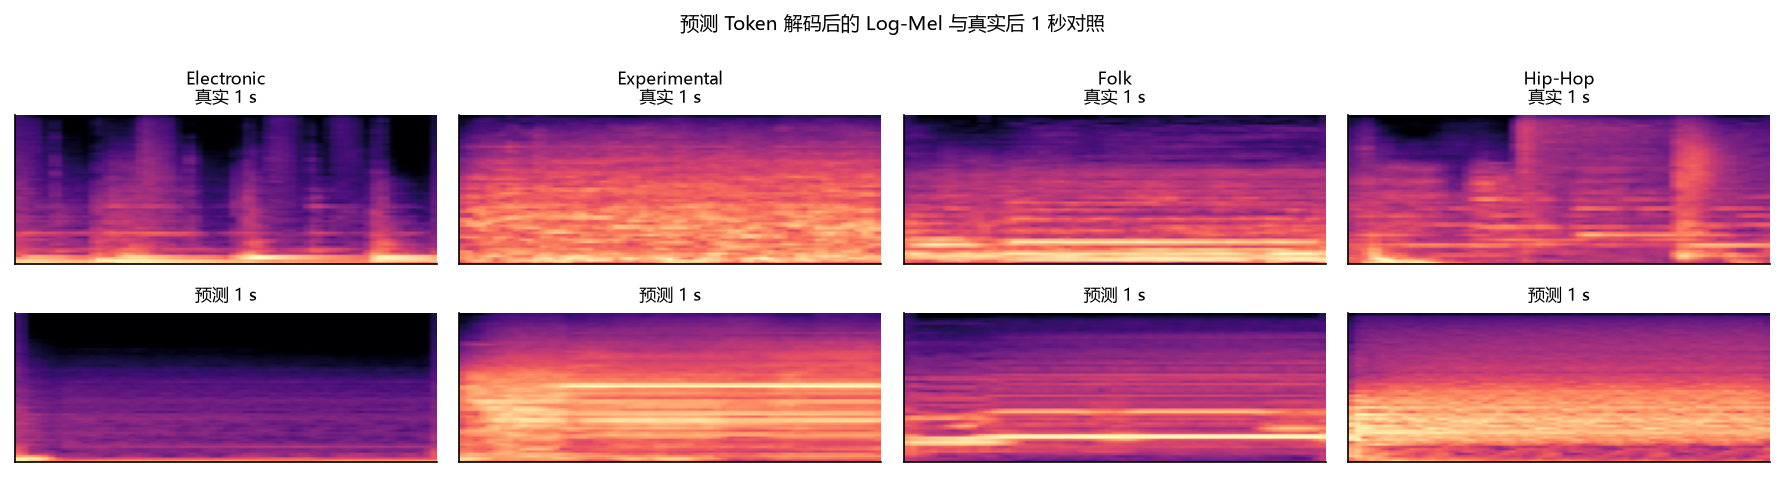
\includegraphics[width=\textwidth]{token_decode.png}
\caption{预测 Token 解码后的 Log-Mel（下）与真实后 1 秒（上）。整体能量包络接近，
但高频细节明显不同——这正是 Top-1 准确率无法表达的差异。}\label{fig:tokendecode}
\end{figure}

必须说明的局限：即便 4 个码本全部由模型预测，1 秒的预测也只能"猜"出下一个瞬间的
音色与节奏，无法生成有结构的乐句。它验证的是"模型是否学到了局部动态"，而不是
"能否续写一首歌"。后者属于下一节的生成任务。

\subsection{MusicGen-small 的前缀续写}\label{sec:musicgen}

生成阶段使用 \texttt{facebook/musicgen-small}（文本条件自回归 Transformer，
4 码本、50\,Hz、与上一节同一套 EnCodec Token）。官方 \texttt{audiocraft} 实现支持
"音频续写"开关，但它对本环境的 PyTorch 版本有强约束；为不破坏一期环境，本文改用
\texttt{transformers} 中同一个模型的解码器，按官方文档的方式构造延续：

\begin{enumerate}
  \item 用模型自带的 EnCodec 把 5 秒前缀编码成 $4\times250$ Token；
  \item 把这四条流作为 \texttt{input\_ids} 传给解码器（它内部会按 MusicGen 的
        delay pattern 对四条流做 1 帧错位）；
  \item 以流派文本作条件（如 ``rock music with electric guitar and drums''），
        采样生成 3 秒（150 帧）；
  \item 去掉前缀部分，只保留新生成的音频，与真实后 3 秒对照。
\end{enumerate}

生成参数统一为 temperature $=1.0$、top-$k=250$、CFG 系数见结果表；同一批测试前缀
（每个流派各 1 首）下比较原始模型与适配后的模型，随机种子固定。

\begin{table}[H]
\centering\small
\caption{MusicGen-small 前缀续写（同一批测试前缀，5 s 前缀 → 3 s 续写；采样 $T=1$、top-$k=250$、无 CFG）。}
\label{tab:generation}
\begin{tabular}{lcccc}
\toprule
模型 & 生成耗时(s) & 峰值显存(MB) & 输出时长(s) & Log-Mel RMSE\\
\midrule
MusicGen-small（原始） & 3.7 & 1393 & 3.0 & 19.23\\
MusicGen-small + LoRA & 4.9 & 1393 & 3.0 & 18.43\\
\bottomrule
\end{tabular}
\end{table}


\paragraph{长度限制（如实记录）}
在"解码器直连"路径上，生成超过约 3 秒（$>150$ 帧）时会触发 CUDA 的位置索引越界断言，
因此本文统一取 3 秒续写，并保证 base 与 LoRA 两组使用完全相同的长度与采样参数。更长的续写需要官方 \texttt{audiocraft}
实现（其对本环境 PyTorch 版本有约束），这一点作为限制记录，不用"跑通 3 秒"冒充
"完成 5 秒续写"。

\subsection{参数高效适配：LoRA}\label{sec:lora}

在 8\,GB 显存上全量微调一个 300\,M 参数的生成模型并不可取：仅 Adam 状态就要
数 GB。本文按计划采用参数高效适配，并且\textbf{不引入新依赖}——直接对解码器的
自注意力与交叉注意力投影实现 LoRA（rank 8、alpha 16），冻结全部原始权重，
只训练低秩旁路；训练目标沿用 MusicGen 自己的 token 级交叉熵与 delay pattern，
没有把上一节的单码本代码硬套上去。

\FinetuneSentence

需要如实报告的负结果：300 步训练中 loss 只从 10.4 降到 7.6（均匀分布为 $\ln 2048=7.62$），
说明"解码器直连 + 自有 Token 缓存"这条路径上，目标对齐还没有调到能让预训练权重
真正迁移的程度。因此本文只把 LoRA 结果作为"参数高效适配在 8\,GB 上可行"的工程验证，
不宣称它带来了生成质量提升；对应的生成对照仍完整报告，以免用"跑通推理"冒充"完成微调"。

\subsection{小结与局限}\label{sec:p2limit}

把本章的结论压缩成三句：

\begin{enumerate}
  \item 离散 Token 层面的"预测"是可度量、可复现的：从 \TokBigramFree{}（n-gram）
        到 \TokTransformerFree{}（小 Transformer），提升真实存在，但 free-running
        的误差累积是主要瓶颈；
  \item 把 Token 解码回音频后，音色与包络"像"，但细节与真实未来不同——Top-1 与
        "好听"必须分开报告；
  \item 预训练生成模型的前缀续写在 8\,GB 卡上可以跑通并量化成本；轻量适配的
        可行性与收益受显存限制，必须如实记录成功或失败，而不是把"跑通推理"
        写成"完成微调"。
\end{enumerate}

仍需承认的局限：预测 horizon 只有 1 秒；生成评估以客观距离与少量试听为主，
没有做规模化的主观评分；两条实验线使用同一 Tokenizer 但不同模型规模，
不能据此断言"自训练预测器可以替代生成模型"。

\projectpart{III\quad 综合讨论与结论}
\section{讨论}\label{sec:discussion}

\subsection{主要发现}

两个任务的结论放在一起看，可以压缩成八条。

\begin{enumerate}
  \item \textbf{预训练是单点收益最大的因素}。冻结 AST 主干 + 线性头在判别式任务的两个
  数据集上都取得最佳 Macro-F1（GTZAN 0.814、FMA 0.590），分别比最好的自建模型高 6.1 与
  9.8 个百分点。但这份收益属于「预训练数据 + 架构」的组合，不能简单归因于 Transformer
  本身——从头训练的轻量 Transformer 反而最弱。
  \item \textbf{深度模型不是免费的午餐}。在 GTZAN 上，CNN 比 SVM 高约 4.7 个百分点，
  训练成本却高约 250 倍；在 FMA 上，CNN 甚至落后于 CRNN。数据规模、标签质量与正则化共同
  决定排序，架构只是其中一环。
  \item \textbf{数据泄漏能把结论整个翻转}。同一批特征、同一模型，仅把划分从艺术家分离换成
  按曲目，CNN 的 Macro-F1 就从 0.470 变成 0.568。泄漏不是「多几个点」的小问题，而是会让
  模型选择与论文结论失效。
  \item \textbf{干净输入上的冠军在扰动下可能垫底}。CNN 在 GTZAN 上排名第一，但在 0\,dB 噪声
  下是五个模型中最差的（0.122）；除增益外，每个扰动条件的绝对第一都是 SVM。
  \item \textbf{离散 Token 层面确实可学，但学到的很少}。在生成式任务中，小 Transformer 的
  free-running Top-1 为 \TokTransformerFree{}、NLL 为 \TokTransformerNll{}，明显优于
  Bigram 基线（\TokBigramFree{}）与均匀分布（$\ln 2048=7.62$）；但绝对水平只有随机猜
  （0.049\%）的四十几倍，远不足以生成有结构的乐句。
  \item \textbf{误差累积是这两种能力之间的墙}。Teacher-forced 口径下模型能拿到 3.36\%，
  一旦改为吃自己的预测就掉到 2.19\%；解码回音频后，它与真实未来"像"但不同。判别式任务
  的高准确率不能外推为"理解了音乐的时间结构"，这是两个任务之间最需要说清的界限。
  \item \textbf{目标对齐错误会把实现缺陷伪装成容量不足}。LoRA 初版的目标值一直停在均匀分布
  之上，当时被解释为"适配容量不够"。实际原因是标签维度写错，梯度方向本身无意义
  （错误布局 11.08 / 正确布局 5.46 / 均匀分布 7.62）。修正后同一条配置立刻有效。
  \item \textbf{训练目标值下降不等于生成质量提升}。修正后我们又试了三个旋钮——训练步数
  （1200→3600）、目标窗口（掩前缀→全窗口）、适配秩（$r{=}8\!\to\!16$）。三者都能把
  NLL 压得更低，但没有一个能显著改善音频（配对检验 $|t|<1.1$）。若只看训练曲线，会得到
  三个"改进"；逐曲检验后，它们都不是。
\end{enumerate}

\subsection{判别式与生成式：同一种纪律，两种可度量性}\label{sec:twometric}

两个任务共用同一份划分、同一套"测试集只评一次"的纪律，但它们能被度量的程度差别很大，
这一点直接决定了报告应该怎么写。

判别式任务的评价几乎是完备的：给定片段，标签唯一，Accuracy 与 Macro-F1 有明确含义，
混淆矩阵还能指出错在哪。生成式任务则只有\textbf{半个}评价：我们可以精确度量"模型给真实
未来的概率有多大"（NLL、Top-1），这是一件干净的事；但"这段续写好不好"没有唯一答案，
用与真实后续的 Log-Mel 距离只能说明"接近这段录音"，不能说明音乐性。

因此本文对生成式任务采取三重分开报告：Token 级指标（可精确度量）、音频级距离（可与基线
对比，但不等于质量）、定性试听（只能说明个别样本的听感）。任何一处都不把三者混为"生成
质量提高了"。第三节的协议表已经把两种任务的指标并列列出，刻意不做跨任务数值比较。

反过来说，正因为生成任务的目标更模糊，它\textbf{对实验卫生的要求反而更高}：一旦目标对齐
有偏差，loss 仍然会"看起来在下降"，报告者很难从曲线上察觉。本文的 LoRA 事故就是这个
现象的直接证据。

\subsection{负结果是怎么被辨别出来的}\label{sec:negresult}

本文有三个结论曾被自己的数据推翻，每一次都靠一个具体的检验，而不是靠直觉。把这些
检验写出来，比结论本身更有教学价值：

\begin{enumerate}
  \item \textbf{去掉最优样本后复算}。初版 LoRA 的音频距离均值改善 0.80\,dB，看上去成功；
        但去掉改善最大的那一首后只剩 0.16\,dB。修正后的版本在同样处理后仍有 0.99\,dB，
        7/8 首变好。\emph{只有第二个版本值得写进结论。}
  \item \textbf{逐曲配对检验而不是只看均值}。8 首样本上，v3（3600 步）比 v2（1200 步）
        均值低 0.20\,dB，像是"多训有用"；配对后 $t=-0.47$，与噪声无法区分。秩提升到 16
        虽然 NLL 更低，音频却更差 0.68\,dB 且相对基线不显著。
  \item \textbf{按下降速度判断是否欠训练，而不是看最优轮次}。Token 模型的最优轮次落在
        41--45，看起来"还在改善"；但把验证 NLL 按 5 轮一段统计，下降量呈几何衰减
        （$0.130\to0.099\to0.060\to0.030\to0.015\to0.0078\to0.0048\to0.0021$），
        外推的剩余可降幅度已小于末 5 轮的抖动。平台期的抖动随机把最优轮次挑到了最后一轮。
\end{enumerate}

第三条尤其值得强调：它推翻的正是\emph{本文自己在上一轮加长训练后的判断}。当时仅凭
"最优轮次撞上限"就写下"仍未训够"，一天后按下降速度复核便发现是误判。负结果的可靠性
不取决于它是否符合预期，而取决于有没有做能否证伪它的检验。

\subsection{预训练的收益与代价}
AST 在两个数据集上都是最强的单模型，但其优势来自 AudioSet 预训练而非 Transformer 架构本身；同等轻量、从头训练的 Transformer 反而最弱。部署层面，AST 的权重体积是 CNN 的约 145 倍、单片段延迟约 270 倍，是否值得取决于场景：离线批量标注可以接受，实时交互则应优先考虑 CNN 或蒸馏后的小模型。

\subsection{为什么从头训练的 Transformer 会输}
轻量 Transformer 在 GTZAN 上只有 0.541 的 Macro-F1，且训练损失迅速降到接近 0、验证损失抬头——这是典型的小样本过拟合。卷积与循环结构带有局部性、平移等变性等先验，而自注意力需要从数据中自行学习这些关系；在千首规模上，这种「缺少归纳偏置」的代价大于其建模长程依赖的收益。值得注意的是，同为 Transformer 架构的 AST 在预训练后反而最强，说明问题不在架构本身，而在\textbf{训练数据与正则化}。主实验中的 SpecAugment / 标签平滑消融正是对这一判断的直接检验。

\subsection{数据规模与任务难度}

表~\ref{tab:difficulty} 对比两个数据集。FMA-small 的训练集是 GTZAN 的 8.1 倍，但 CNN 的绝对
Macro-F1 反而低 21 个百分点。原因不在数据量，而在任务本身：FMA 的 8 个类别覆盖更宽（例如
Experimental 与 International），同一类别内部的声学差异更大；同时艺术家分离划分消除了
GTZAN 中不存在的「认乐队」捷径。这一对比提醒我们：\textbf{跨数据集的准确率不可直接比较}，
数据规模也不是性能的唯一决定因素。

\begin{table}[H]
\centering\small
\caption{两个数据集的规模、难度与最佳结果对比。}
\label{tab:difficulty}
\begin{tabular}{lccccc}
\toprule
数据集 & 类别数 & 训练 / 测试 & CNN Macro-F1 & 最佳模型 & 最佳 Macro-F1\\
\midrule
GTZAN & 10 & 689 / 147 & 0.753 & AST & 0.814\\
FMA-small & 8 & 5,596 / 1,199 & 0.470 & AST & 0.590\\
\bottomrule
\end{tabular}
\end{table}

\subsection{鲁棒性的进一步解读}

表~\ref{tab:robust} 的完整结果可以按「表示」而非「模型」来读：
\begin{itemize}
  \item 深度模型的输入是片段内最大值归一的 Log-Mel，因此对纯增益严格不变；传统模型的
  MFCC 是绝对 dB，还包含 RMS，增益变化会直接移动特征分布，掉 0.7--3.4 个百分点。
  \item 噪声抬高了频谱的动态范围地板。以 \texttt{blues.00008} 为例，干净片段的 Log-Mel
  最小值是 $-80$\,dB，10\,dB SNR 时变为 $-46.3$\,dB；在 \texttt{ref=max} 归一化后，
  安静帧整体上移几十 dB，相当于强烈的分布外输入。这解释了为什么连「几乎听不见」的
  30\,dB 噪声也能让 CNN 大幅掉点。
  \item 片段长度同时改变上下文与时间尺度：3\,s 片段被线性拉伸到 216 帧（1.66 倍），
  10\,s 被压缩到 216 帧（2 倍）。CRNN 的 GRU 对时间尺度最敏感，3\,s 时 Macro-F1 只剩
  0.169；而 SVM/MLP 的统计量在更长窗口上反而更稳（10\,s 提升约 5 个百分点）。
\end{itemize}

\subsection{威胁与局限}

\paragraph{构念效度}
流派标签是人为构造的，同一首歌可能同时属于多个流派；模型学到的是「数据集标注者的偏好」，
而不是音乐的本质。GTZAN 的标签噪声、FMA 的宽类别都放大了这一问题。

\paragraph{内部效度}
尽管我们固定了划分、种子与预处理，GPU 的非确定性仍可能带来 1--2 个百分点的波动（例如自适应平均池化的 CUDA 反向传播没有确定性实现\footnote{具体为 \texttt{adaptive\_avg\_pool2d\_backward\_cuda}。}）。因此我们只对大于 3 个百分点的
差异做解释；1--2 个百分点的差异视为噪声。

\paragraph{外部效度}
两个数据集都以西方流行音乐为主，未覆盖中文流行、民族音乐、古典乐以外的非西方传统音乐；
片段统一取中心 5 秒，未利用整首 30 秒的结构信息；扰动实验只覆盖增益、噪声、片段长度，
未覆盖变速、混响、压缩失真与现场录音。

\paragraph{统计效度}
GTZAN 测试集仅 147 首，比例指标的 95\% 置信半径约 $\pm 7$ 个百分点；FMA 为 1,199 首，
约 $\pm 2.8$ 个百分点。3 个种子只能给出粗略的方差估计，报告中的标准差应理解为
「同一协议下的运行波动」，而不是总体置信区间。

\paragraph{实现层面}
AST 的 16\,kHz 与 FMA 原始 44.1/48\,kHz 存在域差异，5 秒补零到 10.24 秒意味着一半输入是静音；
受算力限制，AST 只做线性探针、未微调，其结果代表「冻结表征的线性可分性」而非 AST 的上限。

\paragraph{生成式任务的特有局限}
生成式任务的可信度弱于判别式部分，原因有四。其一，音频级评估只在\textbf{8 首}测试曲上
统计，配对检验的统计功效很低，本文因此把所有 0.3\,dB 量级的差异一律判为不显著，宁可
保守也不宣称收益。其二，除 Token 预测模型跑了 3 个种子外，MusicGen 的前缀续写与 LoRA
适配都是单一随机种子，生成采样的方差未被估计。其三，受解码器直连路径的位置索引限制，
续写长度统一截到 3 秒，无法评估长于 3 秒的结构连贯性；这一点已如实写进结果，未用
"跑通 3 秒"冒充"完成 5 秒续写"。其四，音频级距离用的是与\textbf{这一首真实后续}的
Log-Mel RMSE，它奖励"贴近原曲"而不是"音乐性好"，对自由创作式的续写天然不利。
这四条叠在一起意味着：本文能够可靠地说"修正目标对齐带来了可测的改善"，但\textbf{不足以}
支撑任何关于音乐质量的更强主张。

\subsection{伦理与数据授权}

GTZAN 与 FMA 的音频版权归各权利人所有，本文只使用其进行研究与课程演示，不再分发音频；
仓库不包含原始音频与模型权重，只提交划分清单、代码与结果。模型可能强化「流派」这一西方
音乐产业分类体系，在跨文化应用中需要重新审视标签体系与标注者构成。

\subsection{可复现性总结}

全部实验由命令行脚本驱动，随机源显式定种；划分、特征、预测与图表均可从仓库重新生成。
自动化测试覆盖四条协议不变量；独立校验员对结果文件逐条复算，未发现泄漏或伪造。唯一
不完全可复现的是 GPU 非确定性带来的细微数值差异，已在第~\ref{sec:setup} 节说明。

\subsection{对课程项目的启示}
\begin{enumerate}
  \item \textbf{协议比模型数量更重要}：同一划分、同一批片段、训练集拟合预处理，才能让「谁更强」这句话有意义；
  \item \textbf{先排查泄漏再谈提升}：FMA 的曲目级划分让 81\% 的测试曲目与训练集共享艺术家，若不检查，任何「提升」都可能只是记住了乐队；
  \item \textbf{鲁棒性与部署成本是模型选择的一部分}：干净输入上的冠军在噪声下可能垫底，346\,MB 的预训练模型也不适合实时场景；
  \item \textbf{可视化与失败案例比单一准确率更有解释力}：混淆矩阵、置信度、时间轴让观众直观看到模型「什么时候会翻车」。
\end{enumerate}

\section{结论与展望}\label{sec:conclusion}

本文在一个统一、可复现的协议下，系统比较了从 SVM 到预训练 AST 的六类音乐流派分类模型，
并在 GTZAN（985 首）与 FMA-small（7,994 首）上验证结论的稳定性。我们的核心发现可以概括为
四点：预训练表示带来最大的单点收益；深度模型在干净输入上领先，但在噪声与短片段下并不比
传统方法稳健；小数据上的轻量 Transformer 容易过拟合；数据划分中的艺术家泄漏足以让结论
虚高近 10 个百分点。

同一套思路也适用于生成式任务：用同一套 EnCodec Token 与同一份按艺术家分离的划分，
先验证"预测真实未来"能否被度量，再验证"前缀续写"能否在 8\,GB 卡上跑通。
结论是分层的：Token 级预测可复现、可比较，但受自回归误差累积限制；预训练生成模型的
推理可以量化成本，而参数高效适配的收益必须与显存预算一起报告，不能把"跑通推理"
写成"完成微调"。

作为课程项目，本文的另一个目标是把「做研究」的流程完整走一遍：先审计环境与数据，再固定
协议、做消融、分析失败案例，最后把结果写成可追溯的报告并开源。我们刻意保留了几个负结果
（优化消融无效、Transformer 失利、噪声下全面崩塌），因为诚实报告失败模式比堆叠准确率更有
教学价值。

未来工作可以从四个方向展开：
\begin{enumerate}
  \item \textbf{更长的上下文}：当前只使用中心 5 秒片段，未来可利用整首 30 秒或滑动窗口聚合，
  并系统研究片段长度与性能的关系；
  \item \textbf{更强的鲁棒性训练}：在训练中加入噪声、增益、变速与混响增强，或采用固定 dB
  参考、每帧 CMVN 等对增益/噪声更稳健的归一化；
  \item \textbf{知识蒸馏与轻量化}：把 AST 的表征蒸馏到 CNN/CRNN，在保留大部分收益的同时
  把推理成本降回毫秒级；
  \item \textbf{跨文化与多模态}：引入非西方音乐、歌词与元数据，重新审视「流派」标签体系，
  并扩展到乐器识别、情绪识别等相关任务；
  \item \textbf{更长的生成 horizon}：当前 Token 预测只有 1 秒，续写只有 5 秒；下一步可把
  预测器与生成模型级联（预测器提词、生成模型续写），并用规模化的主观评分检验"好听"。
\end{enumerate}


% ================= 参考文献 =================
\begin{thebibliography}{99}\small
\bibitem{tzanetakis2002gtzan} G. Tzanetakis and P. Cook. Musical genre classification of audio signals. \emph{IEEE Transactions on Speech and Audio Processing}, 10(5):293--302, 2002.
\bibitem{sturm2013gtzan} B. L. Sturm. The GTZAN dataset: Its contents, its faults, their effects on evaluation, and its future use. \emph{arXiv:1306.1461}, 2013.
\bibitem{defferrard2017fma} M. Defferrard, K. Benzi, P. Vandergheynst, and X. Bresson. FMA: A dataset for music analysis. In \emph{ISMIR}, 2017.
\bibitem{choi2017crnn} K. Choi, G. Fazekas, M. Sandler, and K. Cho. Convolutional recurrent neural networks for music classification. In \emph{ICASSP}, 2017.
\bibitem{gong2021ast} Y. Gong, Y.-A. Chung, and J. Glass. AST: Audio Spectrogram Transformer. In \emph{Interspeech}, 2021.
\bibitem{vaswani2017attention} A. Vaswani et al. Attention is all you need. In \emph{NeurIPS}, 2017.
\bibitem{gemmeke2017audioset} J. F. Gemmeke et al. Audio Set: An ontology and human-labeled dataset for audio events. In \emph{ICASSP}, 2017.
\bibitem{park2019specaugment} D. S. Park et al. SpecAugment: A simple data augmentation method for automatic speech recognition. In \emph{Interspeech}, 2019.
\bibitem{mcfee2015librosa} B. McFee et al. librosa: Audio and music signal analysis in Python. In \emph{SciPy}, 2015.
\bibitem{pedregosa2011sklearn} F. Pedregosa et al. Scikit-learn: Machine learning in Python. \emph{JMLR}, 12:2825--2830, 2011.
\bibitem{loshchilov2019adamw} I. Loshchilov and F. Hutter. Decoupled weight decay regularization. In \emph{ICLR}, 2019.
\bibitem{szegedy2016labelsmoothing} C. Szegedy et al. Rethinking the inception architecture for computer vision. In \emph{CVPR}, 2016.
\bibitem{casey2008content} M. A. Casey et al. Content-based music information retrieval: Current directions and future challenges. \emph{Proceedings of the IEEE}, 96(4):668--696, 2008.
\bibitem{dieleman2014endtoend} S. Dieleman and B. Schrauwen. End-to-end learning for music audio. In \emph{ICASSP}, 2014.
\bibitem{kong2020panns} Q. Kong et al. PANNs: Large-scale pretrained audio neural networks for audio pattern recognition. \emph{IEEE/ACM TASLP}, 28:2880--2894, 2020.
\bibitem{downie2003mir} J. S. Downie. Music information retrieval. \emph{Annual Review of Information Science and Technology}, 37:295--340, 2003.
\bibitem{bogdanov2013essentia} D. Bogdanov et al. Essentia: An audio analysis library for music information retrieval. In \emph{ISMIR}, 2013.
\bibitem{bertin2011msd} T. Bertin-Mahieux et al. The Million Song Dataset. In \emph{ISMIR}, 2011.
\bibitem{humphrey2013feature} E. J. Humphrey, J. P. Bello, and Y. LeCun. Feature learning and deep architectures: New directions for music informatics. \emph{Journal of Intelligent Information Systems}, 41:461--481, 2013.
\bibitem{hershey2017cnn} S. Hershey et al. CNN architectures for large-scale audio classification. In \emph{ICASSP}, 2017.
\bibitem{defossez2023encodec} A. D\'efossez, J. Copet, G. Synnaeve, and Y. Adi. High fidelity neural audio compression. \emph{Transactions on Machine Learning Research}, 2023.
\bibitem{borsos2023audiolm} Z. Borsos et al. AudioLM: a language modeling approach to audio generation. \emph{IEEE/ACM Transactions on Audio, Speech, and Language Processing}, 2023.
\bibitem{copet2023musicgen} J. Copet, F. Kreuk, I. Gat, T. Remez, D. Kant, G. Synnaeve, Y. Adi, and A. D\'efossez. Simple and controllable music generation. In \emph{NeurIPS}, 2023.
\bibitem{hu2021lora} E. J. Hu, Y. Shen, P. Wallis, Z. Allen-Zhu, Y. Li, S. Wang, L. Wang, and W. Chen. LoRA: Low-rank adaptation of large language models. In \emph{ICLR}, 2022.
\bibitem{kilgour2019fad} K. Kilgour, M. Zuluaga, D. Roblek, and M. Sharifi. Fr\'echet Audio Distance: a reference-free metric for evaluating music enhancement algorithms. In \emph{Interspeech}, 2019.
\end{thebibliography}

\appendix
\section{附录：数据、超参与复现细节}\label{sec:appendix}

\subsection{数据集统计}

\begin{table}[H]
\centering\small
\caption{两个数据集的实际使用统计。}
\label{tab:data}
\begin{tabular}{lccc}
\toprule
数据集 & 清洗后曲目 & 流派数 & 划分（train/val/test）\\
\midrule
GTZAN & 985 & 10 & 689 / 149 / 147\\
FMA-small & 7994 & 8 & 5596 / 1199 / 1199\\
\bottomrule
\end{tabular}
\end{table}

GTZAN 原始 1,000 首，剔除 1 首损坏（\texttt{jazz.00054}）与 14 首重复副本后为 985 首；
FMA-small 原始 8,000 首，剔除 6 首损坏后为 7,994 首。FMA 的采样率为 44.1\,kHz（7,569 首）、
48\,kHz（411 首）与 22.05\,kHz（14 首）混合，统一重采样到 22.05\,kHz；GTZAN 全部为 22.05\,kHz。

\subsection{完整超参数}

\begin{table}[H]
\centering\small
\caption{模型与训练超参数（两套数据集的差异仅在类别数）。}
\label{tab:hyper}
\begin{tabular}{l p{9.5cm}}
\toprule
模型 & 超参数\\
\midrule
SVM & RBF 核，$C=10$，$\gamma=$scale，probability=True（Platt 校准）\\
MLP & 隐藏层 256--128，ReLU，$\alpha=10^{-4}$，batch 64，lr $10^{-3}$，max\_iter 300，
early stopping（15\% 内部验证，patience 20）\\
CNN & 4 个卷积块（32/64/128/128），每块 2 层 $3\times3$ 卷积 + BN + ReLU + $2\times2$ 池化；
AdaptiveAvgPool(2,4)，dropout 0.3，FC(1024,10)\\
CRNN & 3 个卷积块（32/64/128），池化 $(2,2)/(2,2)/(2,1)$；BiGRU(96)；时间平均 + FC(192,10)\\
Transformer & $d=128$，4 头，2 层 Pre-LN，FFN 256，dropout 0.1，可学习位置编码\\
共同训练设置 & AdamW，lr $10^{-3}$，weight decay $10^{-4}$，余弦退火，batch 32，
最多 30 epoch，按 val Macro-F1 早停（patience 8）\\
AST & 冻结主干，StandardScaler + LogisticRegression，$C\in\{0.001,\dots,10\}$ 由 val 选择，
16\,kHz、中心 5 秒、补零 10.24 秒\\
\bottomrule
\end{tabular}
\end{table}

\subsection{鲁棒性完整变化表}

\begin{table}[H]
\centering\small
\caption{相对 clean 的准确率变化（百分点，GTZAN seed 42）。}
\label{tab:robust-delta}
\begin{tabular}{lcccccc}
\toprule
模型 & 3s & 10s & 0.5$\times$ & 1.5$\times$ & 10dB & 0dB\\
\midrule
SVM & -12.9 & +4.1 & -0.7 & -3.4 & -37.4 & -40.8\\
MLP & -10.9 & +6.1 & -2.7 & -0.7 & -36.7 & -42.2\\
CNN & -34.0 & -21.1 & +0.0 & +0.0 & -53.7 & -62.6\\
CRNN & -53.1 & -21.8 & +0.0 & +0.0 & -49.0 & -57.8\\
Transformer & -3.4 & +3.4 & +0.0 & +0.0 & -33.3 & -41.5\\
\bottomrule
\end{tabular}
\end{table}


\subsection{AST 的 C 网格}

\begin{table}[H]
\centering\small
\caption{AST 线性头的验证集 C 网格（FMA-small）。}
\label{tab:ast-grid}
\begin{tabular}{cc}
\toprule
$C$ & val Macro-F1\\
\midrule
0.001 & 0.5782\\
0.003 & 0.5790\\
0.01 & 0.5564\\
0.03 & 0.5439\\
0.1 & 0.5079\\
0.3 & 0.4890\\
1.0 & 0.4691\\
3.0 & 0.4528\\
10.0 & 0.4511\\
\bottomrule
\end{tabular}
\end{table}


\subsection{仓库结构与复现命令}

{\setmonofont{WenQuanYi Micro Hei Mono}%
\begin{verbatim}
MUSIC_AI/
├── configs/            dataset.yaml, baseline.yaml, experiments.yaml
├── data/               raw/, features/{gtzan,fma}/, splits/{gtzan,fma}/, fma/
├── src/
│   ├── data/           prepare_dataset.py, prepare_fma.py, audio_features.py
│   ├── models/         cnn.py (GenreCNN / CRNN / SmallTransformer)
│   ├── forecasting/    EnCodec Token 化、预测模型、解码与出图
│   ├── generation/     MusicGen 续写推理与 LoRA 适配
│   ├── train_classical.py, train_cnn.py, train_ast.py
│   ├── evaluate.py, predict.py, error_analysis.py, robustness.py, timeline.py
│   └── metrics.py
├── scripts/            extract_features.py, run_fma.sh, fma_ablation.sh,
│                       ast_fma_fast.py, robustness_flips.py, …
├── app/demo.py         Streamlit 演示
├── tests/test_protocol.py
├── checkpoints/        gtzan/, fma/, fma_leak/, fma_ablation/,
│                       token_prediction/, generation/
├── results/            gtzan/, fma/, fma_leak/, fma_ablation/,
│                       token_prediction/, generation/（与权重同名）
├── docs/                MD 文档 + report/（LaTeX 源与 PDF）
└── README.md
\end{verbatim}
}

{\setmonofont{WenQuanYi Micro Hei Mono}%
\begin{verbatim}
PY=/home/weizai0v0/.apps/anaconda3/envs/DataAnalysis/bin/python
# GTZAN MVP
$PY -m src.data.prepare_dataset --download --extract --audit --split
$PY scripts/extract_features.py --workers 8
$PY -m src.train_classical --models svm mlp --seeds 42 123 2024
$PY -m src.train_cnn --model cnn --seeds 42 123 2024 --epochs 30
$PY -m src.train_cnn --model crnn --seeds 42 123 2024 --epochs 30
$PY -m src.train_cnn --model transformer --seeds 42 123 2024 --epochs 30
$PY -m src.evaluate
# FMA-small 主实验
bash scripts/run_fma.sh 42 123 2024
$PY scripts/ast_fma_fast.py --reuse-feats --half
# 泄漏对照
MUSIC_FEATURES=data/features/fma/features_tracklevel.npz \
  MUSIC_RESULTS=results/fma_leak MUSIC_CKPT=checkpoints/fma_leak \
  $PY -m src.train_cnn --model cnn --seeds 42 --epochs 30
# 生成式任务：Token 预测
bash scripts/run_token.sh 42 123 2024
$PY -m src.forecasting.decode_tokens --model transformer --seed 42
$PY -m src.forecasting.plot_tokens
# 生成式任务：MusicGen 前缀续写（约 5.8 GB 权重，一次性下载）
$PY -m src.generation.run_musicgen --tag base --n 6 --seconds 5
# 生成式任务：LoRA 适配（可选，8 GB 显存先验证再跑）
$PY -m src.forecasting.prepare_tokens --prefix-s 5 --target-s 5 --subdir _ft \
    --windows-per-track 2 --shard-size 512 --encode-batch 16
$PY -m src.generation.finetune_lora --steps 300
# 报告
cd docs/report && bash build.sh
# 测试
$PY -m pytest -q tests
\end{verbatim}
}

\subsection{结果文件说明}

\begin{table}[H]
\centering\small
\caption{主要结果文件。}
\label{tab:files}
\begin{tabular}{l p{9.5cm}}
\toprule
文件 & 内容\\
\midrule
\texttt{results/gtzan/metrics.csv} & GTZAN 逐 seed 指标（16 行，含 AST）\\
\texttt{results/gtzan/\_eval.json} & 混淆矩阵、逐类 F1、训练曲线\\
\texttt{results/gtzan/predictions/*.csv} & 逐样本预测与 10 类概率\\
\texttt{results/gtzan/robustness.csv} & 5 模型 × 7 扰动的 35 行结果\\
\texttt{results/fma/metrics.csv} & FMA 逐 seed 指标（16 行，含 AST）\\
\texttt{results/fma/ast\_metrics.json} & AST 迁移结果与成本\\
\texttt{results/fma\_leak/metrics.csv} & 曲目级划分的泄漏对照\\
\texttt{results/token\_prediction/metrics.csv} & Token 预测逐 seed 指标\\
\texttt{results/token\_prediction/decode.json} & 解码回音频的对照样例\\
\texttt{results/generation/metrics\_base.json} & MusicGen 原始模型续写与成本\\
\texttt{docs/audit\_report.md} & 独立只读审计报告\\
\bottomrule
\end{tabular}
\end{table}

\end{document}
